\documentclass{article}
\pdfoutput=1
% if you need to pass options to natbib, use, e.g.:
%     \PassOptionsToPackage{numbers, compress}{natbib}
% before loading neurips_2018

% ready for submission
% \usepackage{neurips_2018}

% to compile a preprint version, e.g., for submission to arXiv, add add the
% [preprint] option:
% \usepackage[preprint]{neurips_2019}

% to compile a camera-ready version, add the [final] option, e.g.:
%\usepackage{neurips_2019}

% to avoid loading the natbib package, add option nonatbib:
%     \usepackage[nonatbib]{neurips_2018}

\usepackage{arxiv}
\usepackage[utf8]{inputenc} % allow utf-8 input
\usepackage[T1]{fontenc}    % use 8-bit T1 fonts
\usepackage{hyperref}       % hyperlinks
\hypersetup{unicode=true,
            pdfborder={0 0 0},
            breaklinks=true,
            colorlinks=true,
            linkcolor=blue,
            citecolor=blue,
            filecolor=blue,
            urlcolor=blue}
\usepackage{url}            % simple URL typesetting
\usepackage{booktabs}       % professional-quality tables
\usepackage{amsfonts}       % blackboard math symbols
\usepackage{nicefrac}       % compact symbols for 1/2, etc.
\usepackage{microtype}      % microtypography
\usepackage{amsmath}
\usepackage{algorithm,algorithmic}
\usepackage{graphicx}
\usepackage{bbm}
\usepackage{caption} 
\usepackage{natbib}
\usepackage{xr}
\externaldocument[]{supplementary_materials}

\captionsetup[table]{skip=10pt}

\newcommand{\aki}[1]{\textcolor{red}{[Aki: #1]}}

\newcommand{\fracpartial}[2]{\frac{\partial #1}{\partial  #2}}
\newcommand{\Dir}[0]{\textrm{Dirichlet}}
\newcommand{\Ray}[0]{\textrm{Rayleigh}}
\newcommand{\gam}[0]{\textrm{Gamma}}
\newcommand{\dgamma}[0]{\textrm{Gamma}}
\newcommand{\dpoisson}[0]{\textrm{Poisson}}
\newcommand{\dbeta}[0]{\textrm{Beta}}
\newcommand{\dbern}[0]{\textrm{Bernoulli}}
\newcommand{\dunif}[0]{\mathrm{Uniform}}
\newcommand{\dgig}[0]{\textrm{GIG}}
\newcommand{\dnormal}[0]{\mathrm{Normal}}
\newcommand{\dt}[0]{\mathrm{t}}
\newcommand{\igamma}[0]{\textrm{Gamma}^{-1}}
\newcommand{\rayl}[0]{\textrm{Rayleigh}}
\newcommand{\Exp}[0]{\textrm{Exponential}}
\newcommand{\Bet}[0]{\textrm{Beta}}
\newcommand{\GEM}[0]{\textrm{GEM}}
\newcommand{\DP}[0]{\textrm{DP}}
\newcommand{\ESS}[0]{\mathrm{ESS}}
\newcommand{\bm}[1]{\boldsymbol{#1}}
\newcommand{\bbeta}{\bm{\beta}}
\newcommand{\bpi}{\bm{\pi}}
\newcommand{\bomega}{\bm{\omega}}
\newcommand{\bgamma}{\bm{\gamma}}
\newcommand{\blambda}{\bm{\lambda}}
\newcommand{\bphi}{\bm{\phi}}
\newcommand{\btheta}{\bm{\theta}}
\newcommand{\bmu}{\bm{\mu}}
\newcommand{\bb}{\bm{b}}
\newcommand{\bk}{\bm{k}}
\newcommand{\bl}{\bm{l}}
\newcommand{\bn}{\bm{n}}
\newcommand{\bw}{\bm{w}}
\newcommand{\bz}{\bm{z}}
\newcommand{\bx}{\bm{x}}
\newcommand{\bX}{\bm{X}}
\newcommand{\by}{\bm{y}}
\newcommand{\bZ}{\bm{Z}}
\newcommand{\bW}{\bm{W}}
\newcommand{\bS}{\bm{S}}
\newcommand{\bH}{\bm{H}}
\newcommand{\Mult}{\textrm{Multinomial}}
\newcommand{\N}{\mathcal{N}}
\newcommand{\NEW}{\textrm{\tiny new}}
\newcommand{\OLD}{\textrm{\tiny old}}
\newcommand{\sigmat}{\sigma^2}
\newcommand{\IBP}{\textrm{IBP}}
\newcommand{\E}{\mathbb{E}}
\newcommand{\V}{\mathbb{V}}
\newcommand{\Eq}{\mathbb{E}_q}
\newcommand{\cL}{\mathcal{L}}
\newcommand{\cB}{\mathcal{B}}
\newcommand{\cC}{\mathcal{C}}
\newcommand{\cV}{\mathcal{V}}
\newcommand{\cHq}{\mathcal{H}_q}
\newcommand{\test}[1]{\mbox{$#1$}^{\small \mbox{test}}}
\newcommand{\alphaW}{\alpha^{(W)}}
\newcommand{\alphaH}{\alpha^{(H)}}
\newcommand{\betaW}{\beta^{(W)}}
\newcommand{\betaH}{\beta^{(H)}}
\newcommand{\gammaW}{\gamma^{(W)}}
\newcommand{\gammaH}{\gamma^{(H)}}
\newcommand{\gammaT}{\gamma^{(\theta)}}
\newcommand{\rhoW}{\rho^{(W)}}
\newcommand{\rhoH}{\rho^{(H)}}
\newcommand{\rhoT}{\rho^{(\theta)}}
\newcommand{\tauW}{\tau^{(W)}}
\newcommand{\tauH}{\tau^{(H)}}
\newcommand{\tauT}{\tau^{(\theta)}}
\newcommand{\muW}{\hat{W}}
\newcommand{\muH}{\hat{H}}
\newcommand{\Var}{\textrm{Var}}
\newcommand{\LF}{\mathrm{Leapfrog}}

\title{$R^*$: A robust MCMC convergence diagnostic with uncertainty using gradient-boosted machines}

% The \author macro works with any number of authors. There are two commands
% used to separate the names and addresses of multiple authors: \And and \AND.
%
% Using \And between authors leaves it to LaTeX to determine where to break the
% lines. Using \AND forces a line break at that point. So, if LaTeX puts 3 of 4
% authors names on the first line, and the last on the second line, try using
% \AND instead of \And before the third author name.

\author{%
	 Ben Lambert\\
	 MRC Centre for Global Infectious Disease Analysis\\
	 School of Public Health\\
	 Imperial College London\\
	 W2 1PG, United Kingdom\\
	 \texttt{ben.c.lambert@gmail.com} \\
	 \And
	 Aki Vehtari \\
	 Department of Computer Science\\
	 Aalto University\\
	 Finland\\
	 \texttt{aki.vehtari@aalto.fi}
}

\begin{document}
% \nipsfinalcopy is no longer used

\maketitle

\begin{abstract}
  Markov chain Monte Carlo (MCMC) has transformed Bayesian model inference over the past three decades: mainly because of this, Bayesian inference is now a workhorse of applied scientists. Under general conditions, MCMC sampling converges asymptotically to the posterior distribution, but this provides no guarantees about its finite sample performance. The predominant method for monitoring convergence is to run multiple chains and monitor individual chains' characteristics and compare these to the population as a whole: if within-chain and between-chain summaries are comparable, then this is taken to indicate that the chains have converged to a common stationary distribution. Here, we introduce a new method for diagnosing convergence based on whether a machine learning classifier model can successfully discriminate the individual chains. We call this convergence measure $R^*$. In contrast to the predominant $\widehat{R}$, $R^*$ is a single statistic across all parameters that indicates lack of mixing, although individual variables' importance for this metric can also be determined. Additionally, $R^*$ is not based on any single characteristic of the sampling distribution; instead using all the information in the chain, including that given by the joint sampling distribution, which is currently largely overlooked by existing approaches. Since our choice of machine learning classifier, a gradient-boosted regression trees model (GBM), provides uncertainty in predictions, as a byproduct, we obtain uncertainty in $R^*$. The method is straightforward to implement, robust to GBM hyperparameter choice, and could be a complementary additional check on MCMC convergence for applied analyses.
\end{abstract}

\section{Introduction}
Markov chain Monte Carlo (MCMC) is the class of exact-approximate methods that has contributed most to applied Bayesian inference in recent years. In particular, MCMC has made Bayesian inference widely available to a diverse community of practitioners through the many software packages that use it as an internal inference engine: from Gibbs sampling \citep{geman1984stochastic}, which underpins the popular BUGS \citep{lunn2000winbugs} and JAGS \citep{plummer2003jags} libraries, to more recent algorithms: for example, Hamiltonian Monte Carlo (HMC) \citep{neal2011mcmc}, the No U-Turn Sampler (NUTS) \citep{hoffman2014no}, and a dynamic HMC variant \citep{betancourt2017conceptual}, which Stan \citep{carpenter2017stan} and PyMC3 \citep{salvatier2016probabilistic} implement. MCMC methods are currently the most effective tools for sampling from many classes of posterior distributions encountered in applied work, and it seems unlikely that this trend will change soon.

Its importance in applied scientists' toolkits means it is essential that MCMC is used properly and with adequate care. A cost of automated inference software is that it is increasingly easy to regard MCMC as oracular: giving uncompromised views onto the posterior. Because of this, software packages (Stan in particular \citep{carpenter2017stan} is a great exemplar of this), go to great lengths to communicate to users any issues with sampling.


The most important determination of whether MCMC has worked is whether the sampling distribution has converged to the posterior \citep{brooks2011handbook}. MCMC methods are thus created because of an asymptotic property: that given an infinite number of draws, their sampling distribution approaches the posterior (under general conditions). Although the guarantees are asymptotic, MCMC estimates can have negligible bias with only a relatively small number of draws.

The predominant diagnostic method for determining whether practical convergence has occurred relies on the fact that the posterior distribution is the unique stationary distribution for an MCMC sampler. Therefore, it would appear that, if an MCMC sampling distribution stops changing, then convergence has occurred. Unfortunately, anyone who uses MCMC knows that it is full of false dawns: chains can easily become stuck in areas of parameter space, and observation over short intervals mean the sampling distribution \textit{appears} converged. Like furious bees trapped in a room of a house \citep{lambertbees}, MCMC samplers may fail to move due to the narrow gaps that join neighbouring areas. With MCMC, absence of evidence of new areas of high posterior density is, time and again, not evidence of their absence.

To combat this curse of hindsight, running multiple, independent chains, which have been initialised at diverse areas of parameter space is recommended \citep{gelman1992inference}. If the chains appear not to ``mix'' -- a term essentially meaning that it is difficult to resolve an individual chain's path from the mass of paths overlaid on top of one another -- they are yet to converge. This approach makes it less likely that faux-convergence will occur due to chains becoming stuck in an area of parameter space, and running multiple chains is standard practice in applied inference \citep{lambert2018Student}. The predominant approach to quantitatively measuring this mixing is to compare each chain's sampling distribution to that of the population of chains as a whole: specifically, $\widehat{R}$ -- the main convergence statistic used -- compares within-chain variance to that between-chains \citep{gelman1992inference}. If these variances are similar, $\widehat{R}\approx 1$, and chains are deemed to have mixed. Recently, Stan has adopted more advanced variations on the original $\widehat{R}$ formula: for example, splitting individual chains in two to combat poor intra-chain mixing \citep{gelman2013bayesian}; and using ranks of parameter draws rather than the raw values themselves to calculate $\widehat{R}$ \citep{vehtari2019rank}. Additionally, there has been more focus on ensuring that the effective sample size (ESS), a measure of sample quality (see, for example, \cite{lambert2018Student}), is sufficient, and accordingly, new measures of this quantity have been proposed \citep{vehtari2019rank} and adopted \citep{carpenter2017stan}. Collectively, these statistics help alert users of MCMC to issues with sampling (that typically echo issues with the model) meaning that all is not hunky dory.

Here, we introduce $R^*$, a new convergence metric. This statistic is built on the intuition that, if chains are mixed, it should not be possible to discern from a draw's value the chain that generated it. Rephrased, it should not be possible to predict the chain that \textit{caused} a draw. In this vein, we use a machine learning (ML) classifier to measure convergence. Specifically, we train a ML classifier to predict the chain that generated each observation. By evaluating the performance of the classifier on a held-out test set, this provides a new convergence metric. To maximise predictive accuracy, our chosen ML classifier naturally exploits differences in the full joint distributions between chains, which means it's sensitive to variations across the joint distribution of target model dimensions unlike most existent convergence diagnostics. Our statistic, unlike its $\widehat{R}$ cousins, is scalar valued for multivariate distributions: one model provides a single $R^*$, whereas $\widehat{R}$ has separate values for each univariate marginal distribution. However, the ML classifier we use can straightforwardly be interrogated to determine which parameters were most important for generating predictive accuracy. For our ML classifier, we use gradient-boosted regression trees \citep{friedman2001greedy,greenwell2019package} (``GBM''), since these are known to perform well for the types of tabular data that our problem presents \citep{chollet2018}. For the types of problem we test, $R^*$ calculation is of a speed comparable to some of the newer $\widehat{R}$ measures calculated (typically $\mathcal{O}$(seconds) to calculate), although for models with 10,000s of parameters and many iterations, the time taken is longer. It is also insensitive to GBM's hyperparameters and provides a measure of convergence robust to various Markov chain pathologies. In addition, since GBMs can output predicted class probabilities, we obtain uncertainty measures for $R^*$, which we find provides a useful summary of MCMC convergence. $R^*$ can straightforwardly be incorporated into existing software libraries to provide a complementary convergence metric alongside more established measures.

The structure of this paper is as follows: in \S\ref{sec:method}, we describe in detail the method for calculating $R^*$ and its uncertainty; in \S\ref{sec:results}, we examine the performance of $R^*$ across a range of scenarios introduced in \cite{vehtari2019rank} and elsewhere. Code for reproducing the analyses is provided at \url{https://github.com/ben18785/ml-mcmc-convergence}.


\section{Method}\label{sec:method}
If Markov chains have not mixed, it is possible to determine to which chain a draw belongs from its value. This is possible if there are differences in the sampling distribution for any dimension, $\theta$, in the target distribution (Fig. \ref{fig:marginal}): in this case, if the marginal distributions differ between chains, this information can be used to predict which chain a draw belongs to. It  is also possible to predict the chain that generated a given draw if there are differences in the joint distribution of two (or more) dimensions of the target, even if the marginal distributions are the same (Fig. \ref{fig:joint}).

\begin{figure}[!htb]
	\centerline{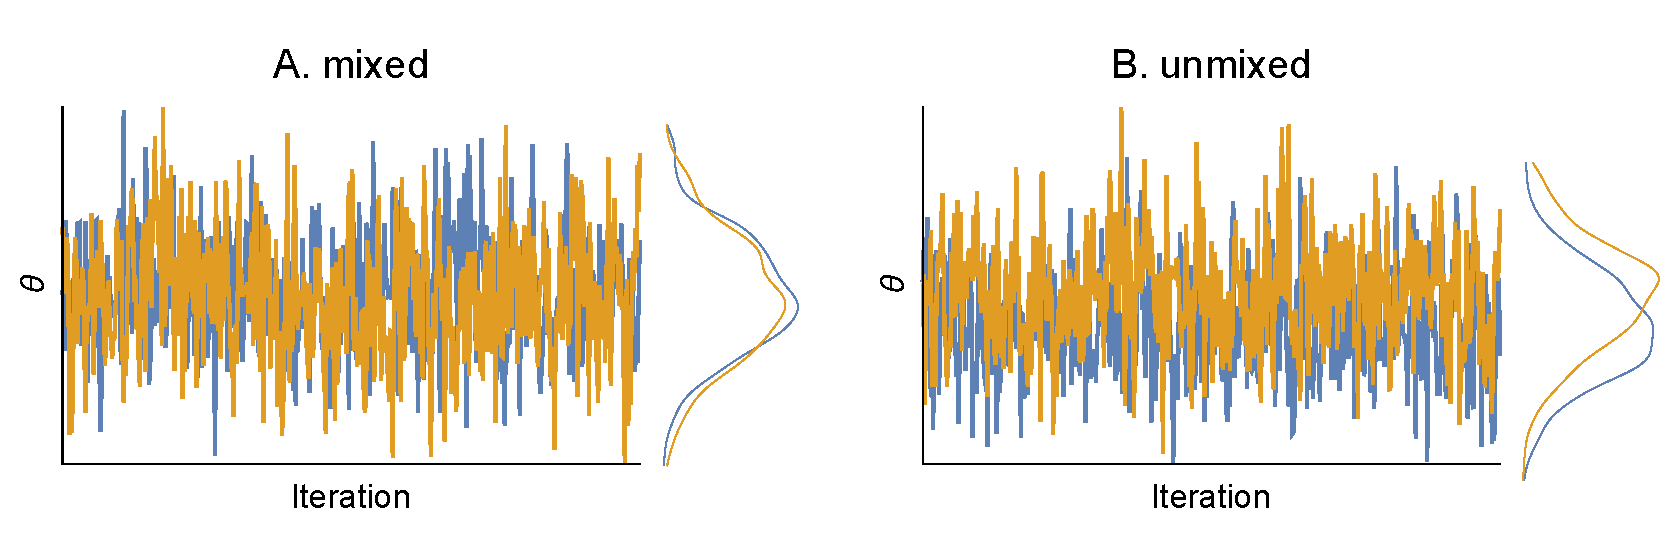
\includegraphics[width=1.0\textwidth]{unmixed_1.pdf}}
	\caption{\textbf{Chain prediction based on the marginal distribution of a single parameter.} A shows the path of two chains that have mixed (with marginal distribution to the right of panel); B shows two chains that have not mixed.}
	\label{fig:marginal}
\end{figure}

\begin{figure}[h]
	\centerline{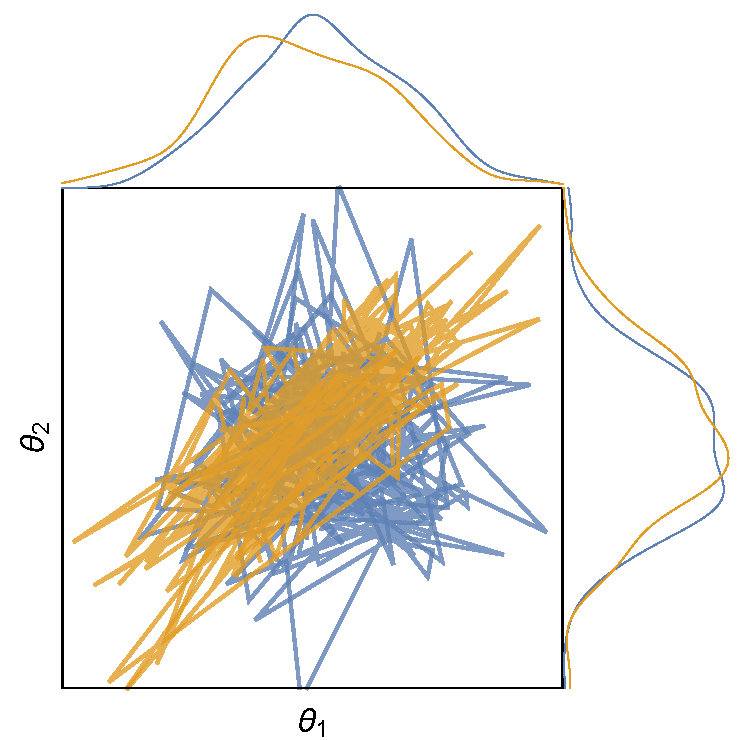
\includegraphics[width=1.0\textwidth]{unmixed_2.pdf}}
	\caption{\textbf{Chain prediction based on the joint distribution of two parameters where each chain's marginals are the same.} A shows the path of two chains that have mixed resulting in similar sampling distributions (to the right and above each panel); B shows two chains that have not mixed.}
	\label{fig:joint}
\end{figure}

These two cases, whilst simple, illustrate the basis of our approach. To determine if a set of Markov chains has converged to the same distribution, we train a supervised machine learning (ML) model to classify the chain to which each draw belongs. By evaluating its performance on a separate test set, we delineate whether chains have mixed based on whether classification accuracy is above the ``null'' case, where accuracy is $1/{N}$, and $N$ is the number of chains. By taking the ratio of ML accuracy to this null accuracy, we obtain a statistic that is interpretable in a similar way to $\widehat{R}$ \citep{vehtari2019rank}. In a nod to this established statistic, we call our statistic $R^*$, and, by design, $R^*\approx 1$ signifies convergence. Algorithm \ref{alg:R_star} gives a recipe for calculating $R^*$.

\begin{algorithm}[tb]
	\caption{$R^*$ calculation}
	\label{alg:R_star}
	\begin{algorithmic}
		\STATE Given chain-wise draws from the target, $\{X^{\{1\}},X^{\{2\}},...,X^{\{N\}}\}$ and a test set length, $S_\text{test}$:
		\FOR{$m=1$ to $N$}
		\STATE Create train and test sets by random-sampling (w/o replacement), $X^{\{m\}}\rightarrow\{X^{\{m\}}_\text{train},X^{\{m\}}_\text{test}\}$
		\ENDFOR
		\STATE Stack $X_\text{train} = (X^{\{1\}}_\text{train},X^{\{2\}}_\text{train},...,X^{\{N\}}_\text{train})^T$
		\STATE Stack $X_\text{test} = (X^{\{1\}}_\text{test},X^{\{2\}}_\text{test},...,X^{\{N\}}_\text{test})^T$
		\STATE Train ML model to classify chain id from any draw, $x$: $\text{ML}(x|X_\text{train}) \rightarrow c$
		\FOR{$s=1$ to $S_\text{test}$}
		\STATE Obtain test draw, $x^{\{s\}}=X_\text{test}(s)\in \mathbb{R}^K$
		\STATE Predict chain id, $c^{\{s\}} = \text{ML}(x^{\{s\}}|X_\text{train})$
		\STATE Compare with actual id, $c^s$: $a^{\{s\}}=\mathbbm{1}(c^{\{s\}}=c^s)$
		\ENDFOR
		\STATE Calculate predictive accuracy, $\bar{a} = \frac{1}{S_\text{test}} \sum_{s=1}^{S_\text{test}} a^{\{s\}}$
		\STATE Calculate ratio to null model accuracy, $R^* = \bar{a} / (1 / N) = N \bar{a}$
		\RETURN $R^*$
	\end{algorithmic}
\end{algorithm}

The ML classifier we use here is a gradient-boosted regression tree (also known as a type of gradient-boosted machine or GBM, introduced in \cite{friedman2001greedy}), which experience has dictated to be a highly predictive framework for use in tabular data \citep{chollet2018} like ours. Specifically, we use the GBM implementation in \textbf{\textsf{R}}'s ``Caret'' package \citep{kuhn2008building}, which, in turn, uses the ``gbm'' package \citep{greenwell2019package}. The data for each chain has dimensions: $X\in \mathbb{R}^{S}\times \mathbb{R}^{K}$, where $S$ is the number of draws taken (here assumed the same for each chain, but this is not a binding constraint), and $K$ is the number of parameters. We split each chain's draws into randomly divided training and testing tests: here, we use 70\% of draws for training and 30\% for testing. Our GBM was rapid to execute training then prediction on the testing set (taking $\mathcal{O}$(seconds) on a desktop computer for both these steps for most models we consider in \S\ref{sec:results}), and its predictive performance was insensitive to its hyperparameters (although we explore this in \S\ref{sec:heterogeneity_robustness}). Unless stated otherwise, in the examples explored in \S\ref{sec:results}, the GBM hyperparameter settings we used were: an interaction depth of 3, a shrinkage parameter of 0.1, 10 observations being the minimum required for each node, and that 50 trees would be grown.

From the GBM fit, predicted chain probabilities can also be obtained, which we leverage to produce an uncertainty distribution for $R^*$. Algorithm \ref{alg:R_star_uncertainty} gives a recipe for generating draws from this distribution, which we now elaborate on in words. For each draw, $s$, in our testing set, GBM outputs a simplex of chain probabilities: $\boldsymbol{p}^{\{s\}}=(p_1^{\{s\}},p_2^{\{s\}},...,p_N^{\{s\}})$, which forms a categorical distribution that can be sampled from to yield a unique chain prediction, $c^{\{s\}}$. By comparing this classification to the true classification, $c^s$, we obtain a binary measure, $a^{\{s\}}=\mathbbm{1}(c^{\{s\}}=c^s)$, of whether this prediction was correct. We repeat this process for each draw in the testing set, generating $\boldsymbol{a}=(a^{\{1\}},a^{\{2\}},...,a^{\{S_\text{test}\}})$, whose average yields a single $R^{*\{i\}}=N \bar{a}$ estimate for iteration $i$. We then iterate this process, for $i=1,2,...,I$, producing a set of $(R^{*\{1\}},R^{*\{2\}},...,R^{*\{I\}})$, which collectively represent a distribution for $R^*$. 


\begin{algorithm}[tb]
	\caption{Procedure to generate $I$ draws of $R^*$}
	\label{alg:R_star_uncertainty}
	\begin{algorithmic}
		\STATE Given test data $X_\text{test}$, number of chains $N$, number of iterations $I$, and fitted
		\STATE model, $\text{ML}(x|X_\text{train})\rightarrow(p_1,p_2,...,p_N)$:
		\FOR{$i=1$ to $I$}
		\FOR{$s=1$ to $S_\text{test}$}
		\STATE Obtain test draw, $x^{\{s\}}=X_\text{test}(s)\in \mathbb{R}^K$
		\STATE Predict chain id probabilities, $(p_1^{\{s\}},p_2^{\{s\}},...,p_N^{\{s\}})= \text{ML}(x^{\{s\}}|X_\text{train})$
		\STATE Draw a chain id, $c^{\{s\}} \sim \text{categorical}(p_1^{\{s\}},p_2^{\{s\}},...,p_N^{\{s\}})$
		\STATE Compare with actual id, $c^s$: $a^{\{s\}}=\mathbbm{1}(c^{\{s\}}=c^s)$
		\ENDFOR
		\STATE Calculate predictive accuracy, $\bar{a} = \frac{1}{S_\text{test}} \sum_{s=1}^{S_\text{test}} a^{\{s\}}$
		\STATE Calculate ratio to null model accuracy, $R^{*\{i\}} = \bar{a} / (1 / N) = N\bar{a}$
		\ENDFOR
		\RETURN $(R^{*\{1\}},R^{*\{2\}},...,R^{*\{I\}})$
	\end{algorithmic}
\end{algorithm}

\section{Results}\label{sec:results}
To illustrate the versatility of $R^*$, we use a range of examples that demonstrate how this statistic fares across a range of scenarios. Table \ref{tab:results} summarises the examples and provides a rationale for their inclusion. The experiments not detailed in the main text are briefly described in \S\ref{sec:further_experiments} and more fully in the relevant sections given in Table \ref{tab:results}.

\begin{table}[]
	\begin{tabular}{l|l|l}
		\textbf{Example }&  \textbf{Relevance} & \textbf{Section} \\
		\midrule
		Autoregressive & \textbf{Examining $R^*$ and sensitivities to its calculation} & \ref{sec:heterogeneity} \\
		& Detecting heterogeneous chain variance using $R^*$ & \ref{sec:heterogeneity_performance} \\
		& Stochasticity in $R^*$ & \ref{sec:heterogeneity_stochasticity}\\
		& Generating $R^*$ uncertainty measure & \ref{sec:heterogeneity_uncertainty}\\
		& Sensitivity of $R^*$ to number of chains & \ref{sec:heterogeneity_numchains}\\
		& Robustness of $R^*$ to ML model hyperparameters & \ref{sec:heterogeneity_robustness}\\
		\midrule
		Multivariate normals & \textbf{Detecting convergence in joint distributions} &  \ref{sec:multivariate_normal}\\
		& Unconverged joint distribution in bivariate normal & \ref{sec:multivariate_normal_bivariate}\\
		& High correlations between dims in 250D normal  & \ref{sec:multivariate_normal_250}\\
		& Measuring contributions of variables to poor convergence & \ref{sec:multivariate_normal_varimportance}\\
		\midrule
		Cauchy & \textbf{Detecting convergence for long-tailed distributions} & \ref{sec:cauchy}\\
		& Comparing $R^*$ and existing measures to objective convergence & \ref{sec:cauchy_objective}\\
		\midrule
		Eight schools model & \textbf{Hierarchical Bayesian model slow convergence} & \ref{sec:eight_shools}\\
		\midrule 
		Wide multivariate normal & \textbf{Detecting convergence when \# draws $\sim$ \# dims} & \ref{sec:wide}\\
		\midrule
		Non-stationary marginals & \textbf{Detecting time-varying sampling distributions} & \ref{sec:non-stationary}\\
		& Trends in mean across all chains & \ref{sec:non-stationary_chains}\\
		& Trends in mean in a single dimension & \ref{sec:non-stationary_single}\\
		& Trends in covariance & \ref{sec:non-stationary_covariance}\\
		& Sensitivity of $R^*$ to chain persistence & \ref{sec:non-stationary_persistence}\\
		\midrule
		Ovarian and prostate models & \textbf{Bayesian models with many parameters and multimodal posteriors} & \ref{sec:prostate}\\
	\end{tabular}\caption{\textbf{Summarising the example problems and reasons for their inclusion.}}\label{tab:results}
\end{table}

\subsection{Heterogeneity in chain variance: autoregressive example}\label{sec:heterogeneity}
In this section, we show how $R^*$ is able to detect heterogeneous variance across Markov chains. Apart from demonstrating how $R^*$ performs, this section also investigates the sensitivity of this measure: across different training and testing sets (\S\ref{sec:heterogeneity_stochasticity}) and different draws from the ML model predicted probability simplex (\S\ref{sec:heterogeneity_uncertainty}); to differing numbers of chains (\S\ref{sec:heterogeneity_numchains}); and, finally, to the ML model hyperparameters (\S\ref{sec:heterogeneity_robustness}). The experiments we use to study these issues are all of similar form to the following data generating process: four Markov chains are generated, where each samples from an autoregressive order 1 (AR(1)) process of the form,
%
\begin{equation}\label{eq:ar1}
X_t = \rho X_{t-1} + \epsilon_t,
\end{equation}
%
where $\epsilon_t\stackrel{i.i.d.}{\sim}\mathcal{N}(0, \sigma)$, $\rho=0.3$ and $t=1,2,...,2000$. Three of the chains share the same $\sigma=1$, whereas the other chain has $\sigma=1/3$, so that it has $1/3$ of the (unconditional) standard deviation of the others.

\subsubsection{Performance of $R^*$}\label{sec:heterogeneity_performance}
To illustrate the consistency of $R^*$, we perform 1000 replicates where, in each case, we generate four $\{X_t\}$ series as described (i.e. where one chain has a lower variance). We then fit a GBM to a labelled training set. The fitted model is then used to classify draws in an independent test set according to the chain which generated them. For each replicate, we then calculated $R^*$ as described in Algorithm \ref{alg:R_star}.

In Fig. \ref{fig:ar1}A, we show how a GBM fitted to one such replicate dataset classifies observations according to a draw's value. Unsurprisingly, since the fourth chain has a smaller variance, observations close to zero are likely to be classified as being generated by this chain.

In Fig. \ref{fig:ar1}B, we show that $R^*>1$ for all replicates, indicating that the chains had not converged in all cases. In Fig. \ref{fig:ar1}C, we show the rank-normalised split-$\widehat{R}$ as calculated in \cite{vehtari2019rank} for each replicate;  as for $R^*$, this metric indicates the chains had not converged in all replicates (as diagnosed by $R^*<1.01$).

\begin{figure}[!htb]
	\centerline{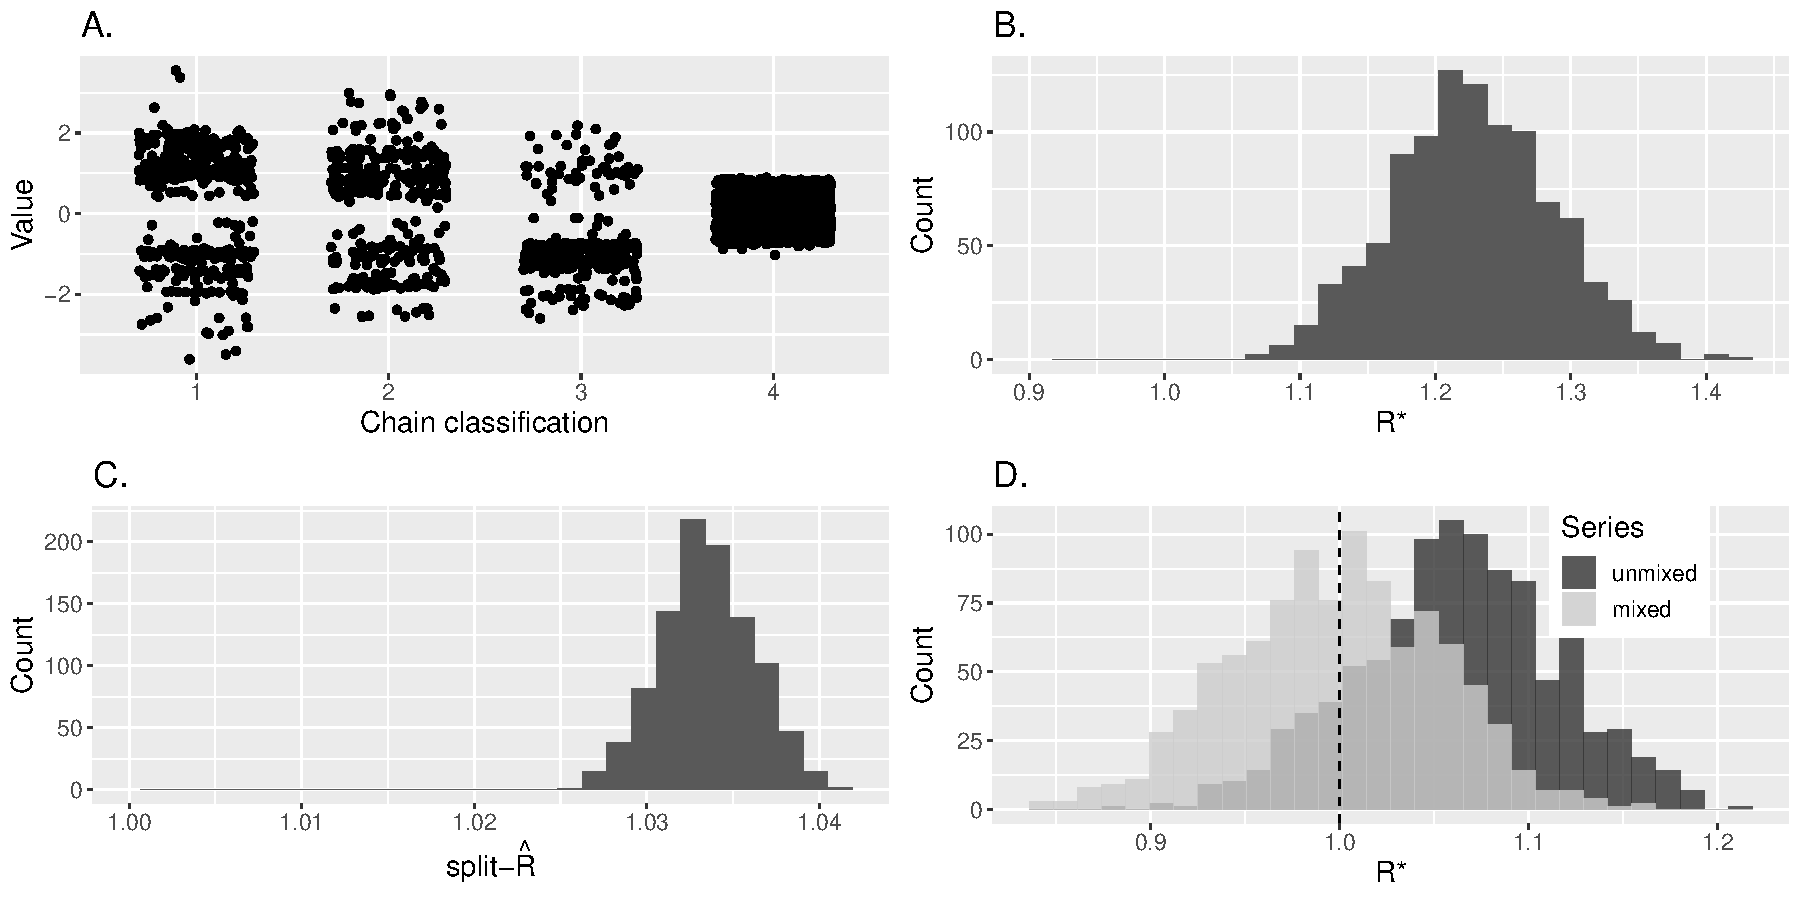
\includegraphics[width=1.0\textwidth]{ar1.pdf}}
	\caption{\textbf{Autoregressive example.} A shows how the GBM's classifications vary according to the draw's value for an example model fit; B shows $R^*$ values generated by Algorithm \ref{alg:R_star} across 1000 replicate datasets; C shows corresponding rank-normalised split-$\widehat{R}$ values as calculated in \cite{vehtari2019rank} for each of the 1000 replicates; and D shows 1000 $R^*$ samples as generated by Algorithm \ref{alg:R_star_uncertainty} for two series: the ``unmixed'' dataset being the same as used for figures A-C; the ``mixed'' where all chains have the same distribution as described in \S\ref{sec:heterogeneity}. Note that, in D, only a single series of each series type is used to generate distribution.}
	\label{fig:ar1}
\end{figure}

\subsubsection{Stochasticity in $R^*$}\label{sec:heterogeneity_stochasticity}
Unlike $\widehat{R}$, $R^*$ is a stochastic convergence measure due to randomness in creating training and testing sets (essentially a form of sampling variation) and randomness in the methods used to train the ML model. This means that even if the same sample is used, $R^*$ will return a different value each time it is calculated if the pseudorandom seed is not fixed. To probe the extent of this randomness, we generated data using the same process as in \S\ref{sec:heterogeneity} but now using varying sample sizes, including samples consisting of 500, 1000, 2000, 4000 and 8000 draws. For each dataset, we computed $R^*$ on it 100 times, allowing the pseudorandom seed to vary between calculations. We stress that, for each sample size, we used the same dataset (so there were 5 datasets created in total -- one for each sample size), so stochasticity comes from $R^*$ calculation, not that from the data generating process.

In Fig. \ref{fig:ar1_samplesize}, we show the results of this study. In this figure, the horizontal axis shows the sample size, and the vertical axis, the value of $R^*$ in each repetition. This shows that as the number of samples increased, variation in $R^*$ declined. At a sample size of 500, there were four cases where $R^*<1$; in larger samples, there were none. Intuitively, the reduction in sampling variation when composing training and test sets from larger samples results in lower variability in ML model predictions. We also expect that larger sample sizes should lead to higher $R^*$ values, since more training data leads to better ML models. We may start to see this here, since the median $R^*=1.25$ at a sample size of 8000 was greater than for the smaller samples. 

If randomness in $R^*$ calculation leads to different conclusions about convergence being drawn, this would be problematic. One potential remedy for this is to repeatedly calculate $R^*$ on a given sample, much as we have done here, and consider the distribution of $R^*$ values computed. The computational cost of doing this may, of course, be unreasonable. Instead, in \S\ref{sec:heterogeneity_uncertainty}, we consider an alternative approach based on bootstrapping a single ML model's predictions.

\begin{figure}[!htb]
	\centerline{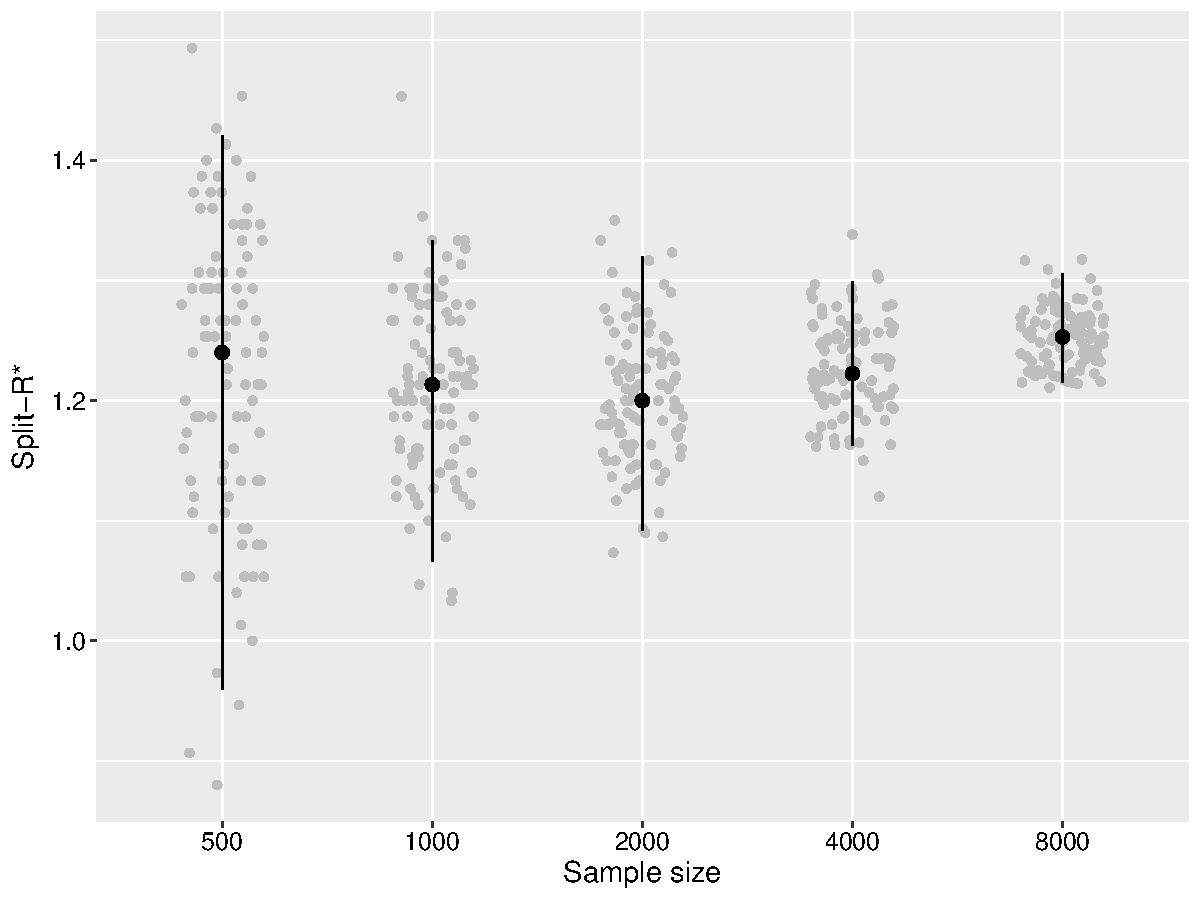
\includegraphics[width=0.6\textwidth]{ar1_samplesize.pdf}}
	\caption{\textbf{Autoregressive example: $R^*$ stochasticity.} The horizontal axis shows sample size; the vertical axis shows the value of $R^*$ calculated as per Algorithm \ref{alg:R_star} applied to chains split into two halves. Grey points show the value of $R^*$ for each replicate (jitter was added to point positions). Black points show the median $R^*$ value; upper and lower whiskers show 2.5\% and 97.5\% quantiles. For each sample size, a single dataset was created and used for all $R^*$ calculations.}
	\label{fig:ar1_samplesize}
\end{figure}

\subsubsection{Uncertainty distribution for $R^*$}\label{sec:heterogeneity_uncertainty}
GBMs return a probability simplex for each draw, indicating the probability that the draw was generated by a given chain. We can use this simplex to generate a measure of uncertainty in $R^*$ as detailed in Algorithm \ref{alg:R_star_uncertainty}. We demonstrate this idea using two datasets: one generated as described in \S\ref{sec:heterogeneity}, where one chain (out of four) has a lower variance than the others (we call this the ``unmixed'' data); and another, where all chains sample from the same distribution (we call this the ``mixed'' data). In Fig. \ref{fig:ar1}D, we show the $R^*$ distributions in each case. For the unmixed data, the distribution has its bulk of mass away from 1, indicating lack of convergence. For the mixed data, the distribution is centred on 1, indicating convergence. In the mixed case, there are many draws where $R^*<1$: these indicate that, in that particular draw from the probability simplex, chain classification is actually worse than selecting a chain identification uniformly at random. Much like how it is possible for $\hat{R}<1$, this is a sample property, driven by the sampling distribution of the categorical distribution defined by the probability simplex.

It is worth emphasising that the uncertainty distribution obtained by Algorithm \ref{alg:R_star_uncertainty} differs from that obtained from repeatedly calculating $R^*$ via Algorithm \ref{alg:R_star} as was done in \S\ref{sec:heterogeneity_stochasticity}. In Algorithm \ref{alg:R_star_uncertainty}, variation in $R^*$ comes from sampling from the probability simplex: if predicted chain probabilities are close to uniform, there will be greater uncertainty in $R^*$. Repeatedly calculating $R^*$ by applying Algorithm \ref{alg:R_star} to the same dataset yields a distribution whose width derives from sampling variation when forming training and testing sets and the stochasticity in training ML models. Collectively, these differences mean that the two measures of uncertainty will differ.

There is an additional difference, though, in the central points of each distribution: the distribution obtained by Algorithm \ref{alg:R_star_uncertainty} will, in general, have a lower mean than that obtained by repeated application of Algorithm \ref{alg:R_star}. To see this, note that the darker-shaded $R^*$ distribution in Figure \ref{fig:ar1}D was generated via Algorithm \ref{alg:R_star_uncertainty} and has a mean around 1.07; the distribution shown in Figure \ref{fig:ar1}B was generated by repeatedly recomputing $R^*$ using Algorithm \ref{alg:R_star} and has a mean closer to 1.22. This difference in mean is expected since predictive performance when assigning chain identities stochastically when sampling from the categorical distribution of the probability simplex (as is done in Algorithm \ref{alg:R_star_uncertainty}) will generally result in worse prediction than when assigning each chain identity using whichever chain has the highest class probability (as is done in Algorithm \ref{alg:R_star}). Of course, we would prefer it if the uncertainty distribution generated by Algorithm \ref{alg:R_star_uncertainty} had a mean closer to the one obtained by repeated application of Algorithm \ref{alg:R_star}. Nonetheless, in practice, we have found that the mean of the $R^*$ distribution generated by Algorithm \ref{alg:R_star_uncertainty} provides a useful cheaper diagnostic.

\subsubsection{Sensitivity to number of chains}\label{sec:heterogeneity_numchains}
We have so far focused on the sensitivity of $R^*$ to chain heterogeneity with a fixed number of chains: four. Since classification becomes a harder problem when there are more categories, we now demonstrate how $R^*$ (as calculated by Algorithm \ref{alg:R_star}) performs across various number of chains. For comparison, we also illustrate how the performance of rank-normalised split-$\widehat{R}$ varies with number of chains. To do so, we consider an autoregressive example similar to that described in \S\ref{sec:heterogeneity}: where all chains bar one have $\sigma=1$, and the remaining chain has $\sigma=1/3$. We consider cases with 2, 4, 8, 16, and 32 chains. The other hyperparameters of the data generating process remain the same as in \S\ref{sec:heterogeneity}.

In Fig. \ref{fig:ar1_numchains}, we show the results of these simulations with 50 replicates at each number of chains. On the horizontal axis, we show the number of chains, and on the vertical axis, the value of each of the two convergence measures ($R^*$ in the left panel; $\widehat{R}$ in the right panel). In general, both measures decline with chain count. For $R^*$, this is because it is harder to classify chains when there are more of them. For $\widehat{R}$, this is because between-chain variance becomes relatively lower to that within them when there are more chains and only one of them differs in its marginal distribution. Across the replicates we ran, median $\widehat{R}<1.01$ for 16 or more chains; a minimum of $R^*=1.10$ was obtained for 32 chains.

The decline of both of these measures when more chains are used hints that perhaps a moving threshold for diagnosing convergence may be pertinent to avoid neglecting those minority of chains with differing information. Here, however, we do not make suggestions on what such guidelines could be and leave this for later work.

\begin{figure}[!htb]
	\centerline{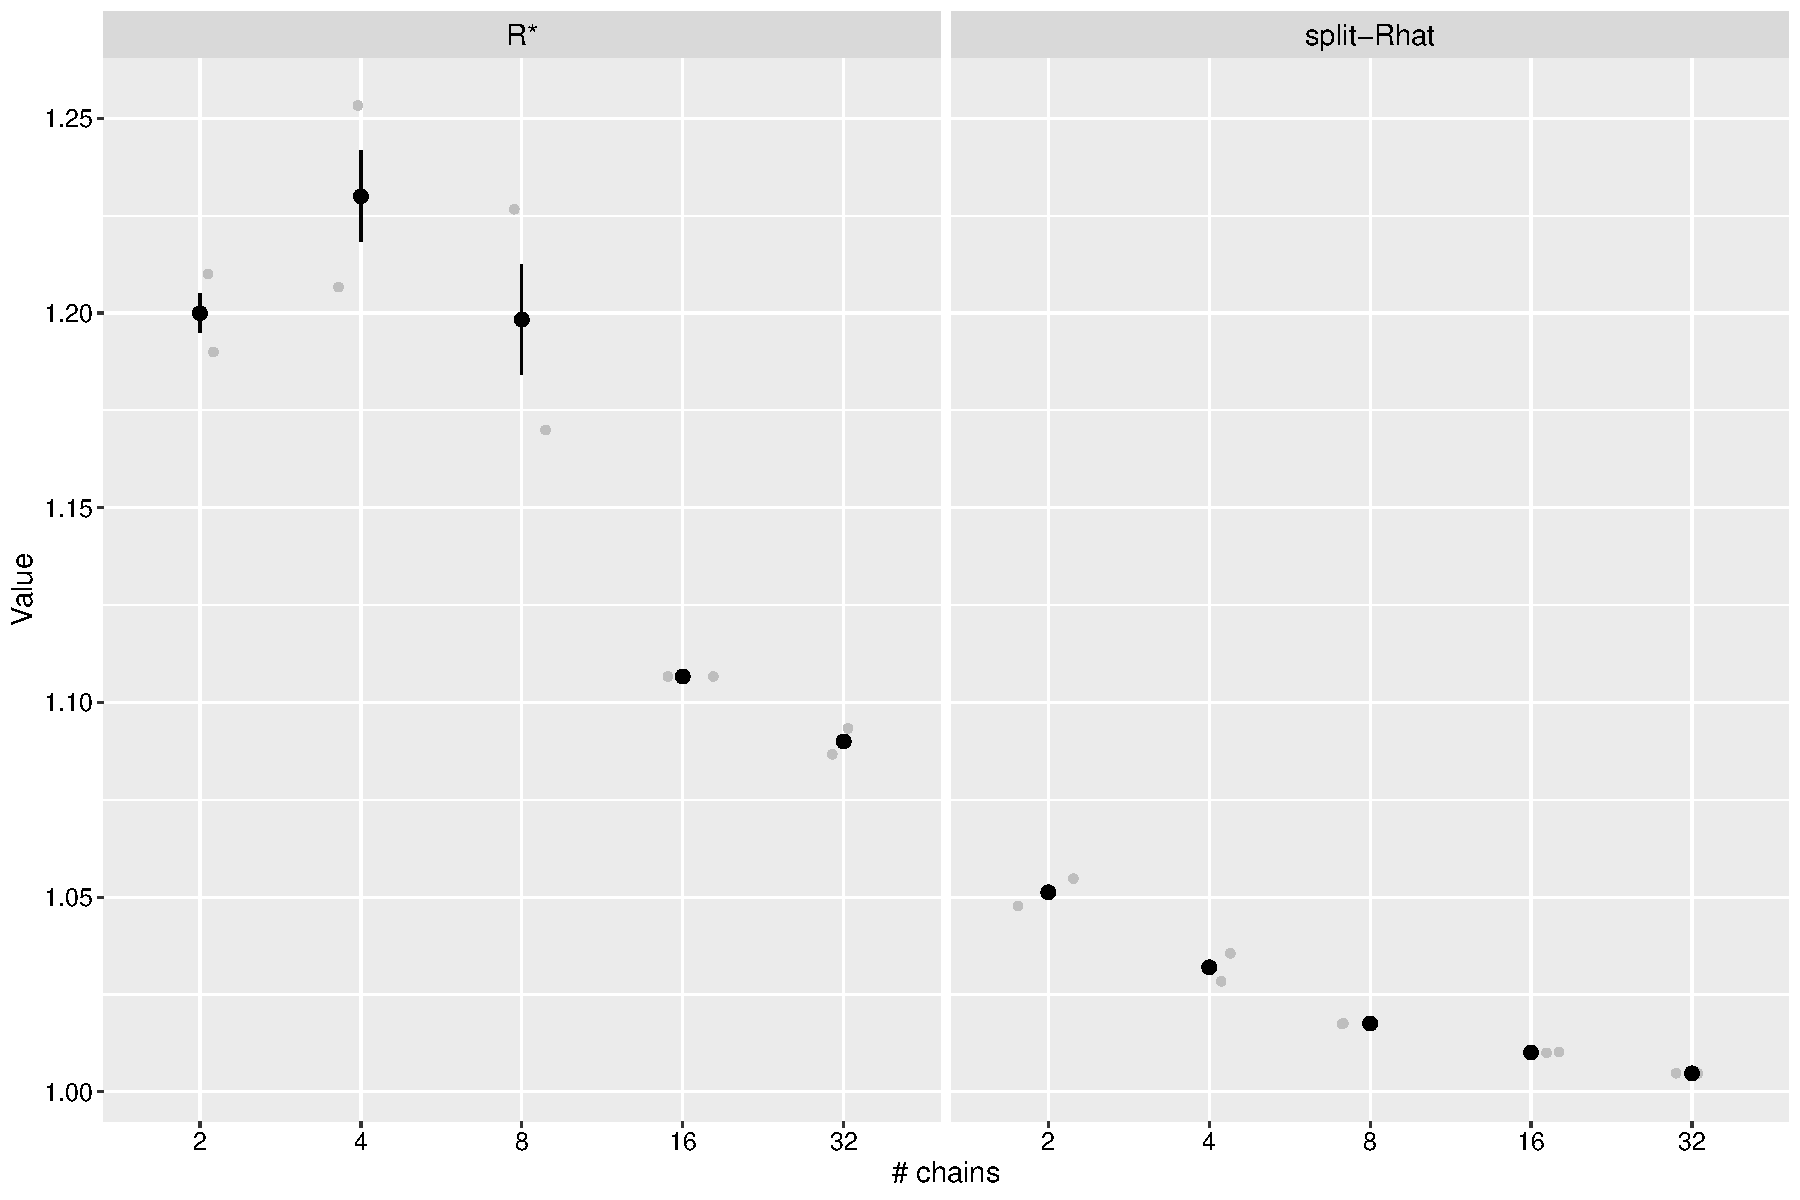
\includegraphics[width=0.8\textwidth]{ar1_numchains.pdf}}
	\caption{\textbf{Autoregressive example: sensitivity to number of chains.} The horizontal axis shows the number of chains used in the data generating process described in \S\ref{sec:heterogeneity_numchains}. The vertical axis shows the value of $R^*$ as calculated by Algorithm \ref{alg:R_star} (left panel) on chains split into two halves, and rank-normalised split-$\widehat{R}$ as calculated in \cite{vehtari2019rank} (right panel). Grey points indicate the values of both convergence measures calculated for each replicate; horizontal jitter has been added to points. The point-ranges shown indicate the 25\%, 50\% and 75\% quantiles across 50 replicates at each number of chains.}
	\label{fig:ar1_numchains}
\end{figure}

\subsubsection{Robustness to hyperparameter choice}\label{sec:heterogeneity_robustness}
The performance of GBM, like all ML methods, depends on its hyperparameters. To investigate the robustness of $R^*$ to GBM hyperparameter choice, we performed a sensitivity analysis. In this, we fit GBMs with six different sets of hyperparameters to replicates consisting of the same data used to generate Fig. \ref{fig:ar1}. The hyperparameters we varied were the interaction depth (3, 5 or 7) and the number of trees (50, 100 or 200). The resultant $R^*$ point estimates across 200 replicates for each hyperparameter setting are shown in Fig. \ref{fig:ar1_sensitivity}. These show that hyperparameter choice affects $R^*$, with the highest median values obtained for an interaction depth of 3 with 50 trees (our default across all the examples we consider in this paper). This analysis does suggest, however, that this effect is relatively minor: indeed, across the various hyperparameter sets considered, the percentage of replicates where $R^*<1$ did not strongly vary.

\begin{figure}[!htb]
	\centerline{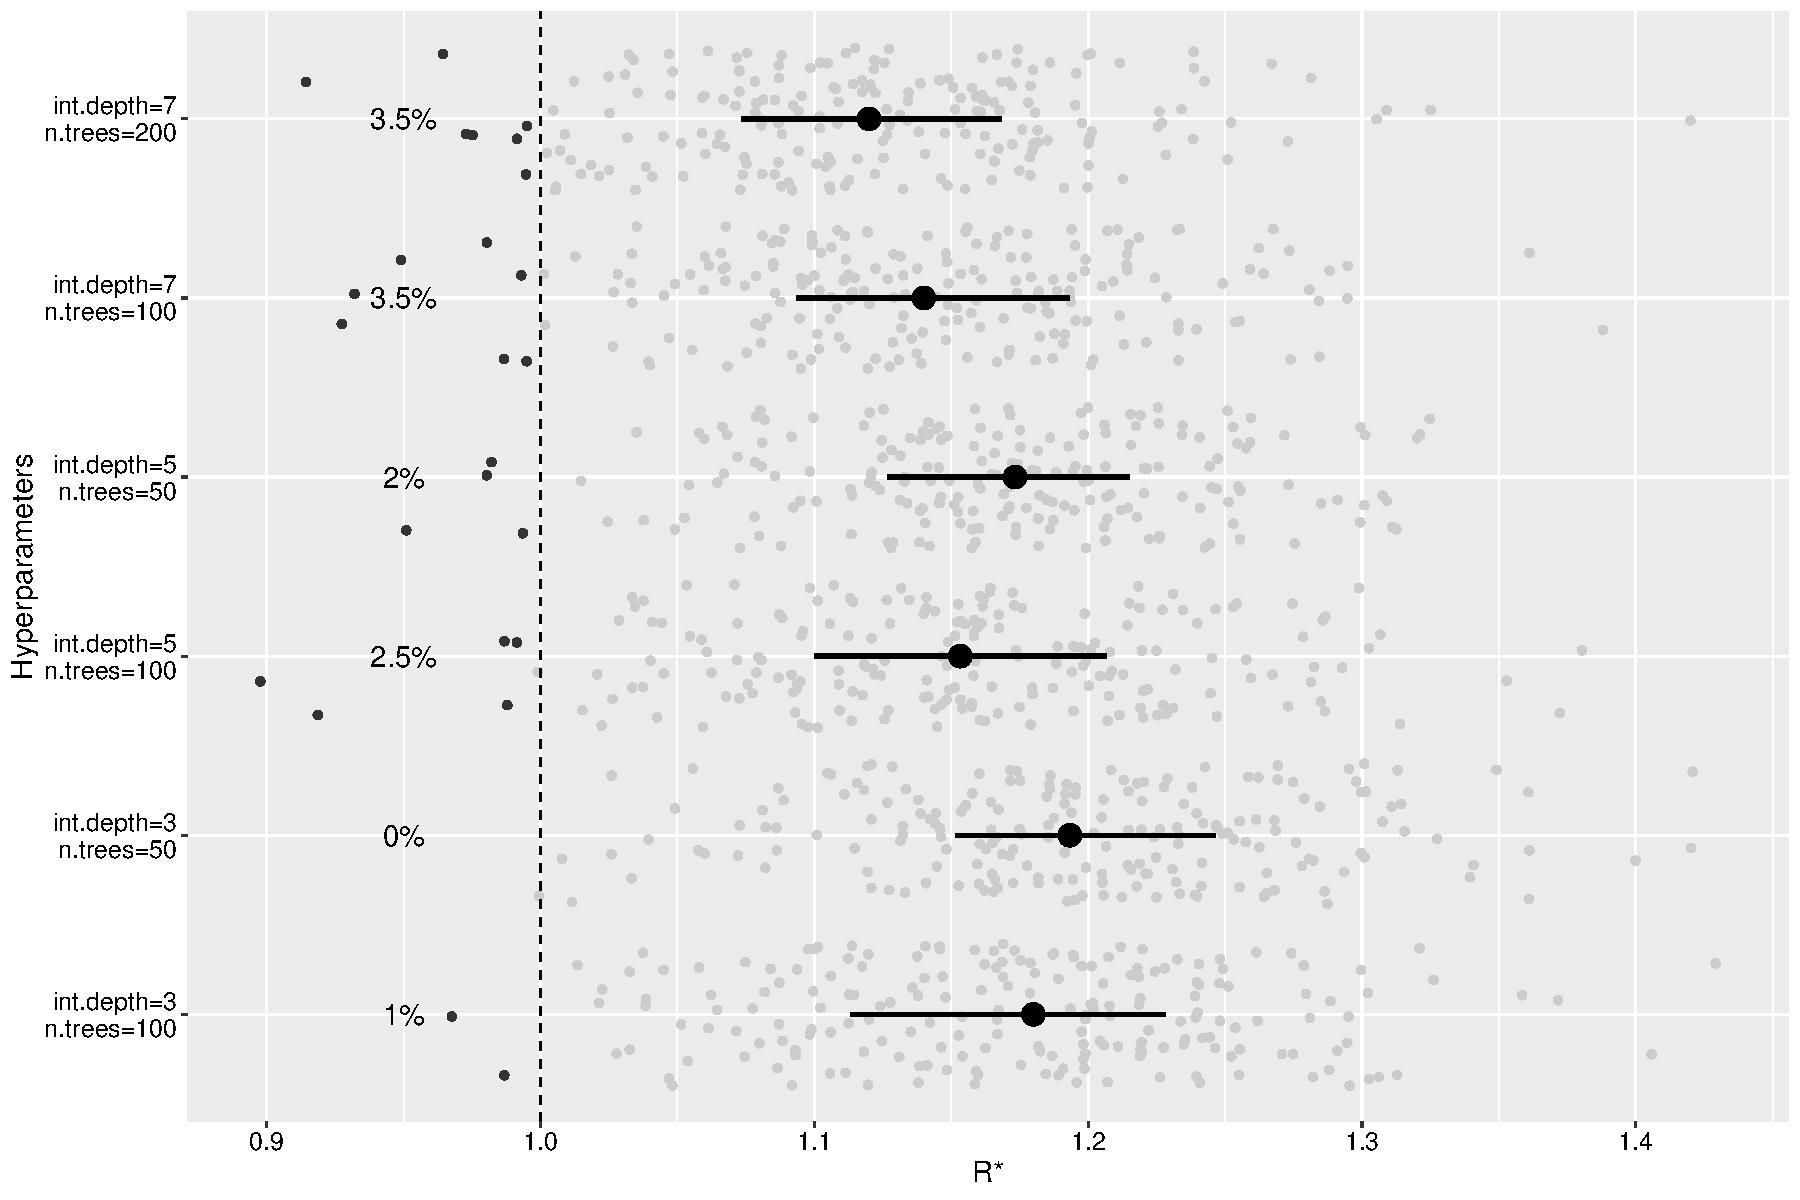
\includegraphics[width=1.0\textwidth]{ar1_sensitivity.pdf}}
	\caption{\textbf{Autoregressive example: sensitivity to GBM hyperparameters.} The rows correspond to GBM models fit using different hyperparameter sets (as indicated for interaction depth and number of trees and using a shrinkage of 0.1 and a minimum observations per node of 10 in all cases). The horizontal axis shows the $R^*$ values generated using Algorithm \ref{alg:R_star} using split chains; points have jitter added and are coloured according to whether they exceed the threshold $R^*=1$, with the percentage below this threshold annotated. The point-ranges shown indicate the 25\%, 50\% and 75\% quantiles for each model.}
	\label{fig:ar1_sensitivity}
\end{figure}

\subsection{Diagnosing convergence in joint distributions: multivariate normal models}\label{sec:multivariate_normal}
In this section, we illustrate how $R^*$ can diagnose convergence issues in the joint target distribution.

\subsubsection{Bivariate model}\label{sec:multivariate_normal_bivariate}
First, we consider a bivariate normal density. In all four chains, we use independent sampling to generate 2000 draws from bivariate normal densities with means of zero; in three of these chains, the covariance matrix is an identity matrix; in one chain, the covariance matrix also has unit diagonal terms but has off-diagonal terms of 0.9, indicating strong covariance between the two dimensions. By construction, all chains target the same marginal distribution in each dimension, but the fourth chain has a different joint distribution.

First, we use the code provided in \cite{vehtari2019rank} to calculate rank-normalised $\widehat{R}$ and two different ESS measures that aim to capture how well certain regions of the posterior have been explored: these are known as bulk-ESS and tail-ESS. In all cases, the various quantities were calculated based on chains split into halves. For both dimensions, the two ESS measures were above 7000, and $\widehat{R}<1.001$, indicating no issues with convergence.

Next, we estimate the $R^*$ distribution using Algorithm \ref{alg:R_star_uncertainty}, which is shown in Fig. \ref{fig:bivariate}. The mean of this distribution is 1.14, and $>$99\% of $R^*$ draws are above 1, indicating that the sampling distribution has not converged. By taking account of all the information in the chains, $R^*$ is able to probe issues in joint distribution convergence which are missed by measures that consider only marginals.

\begin{figure}[!htb]
	\centerline{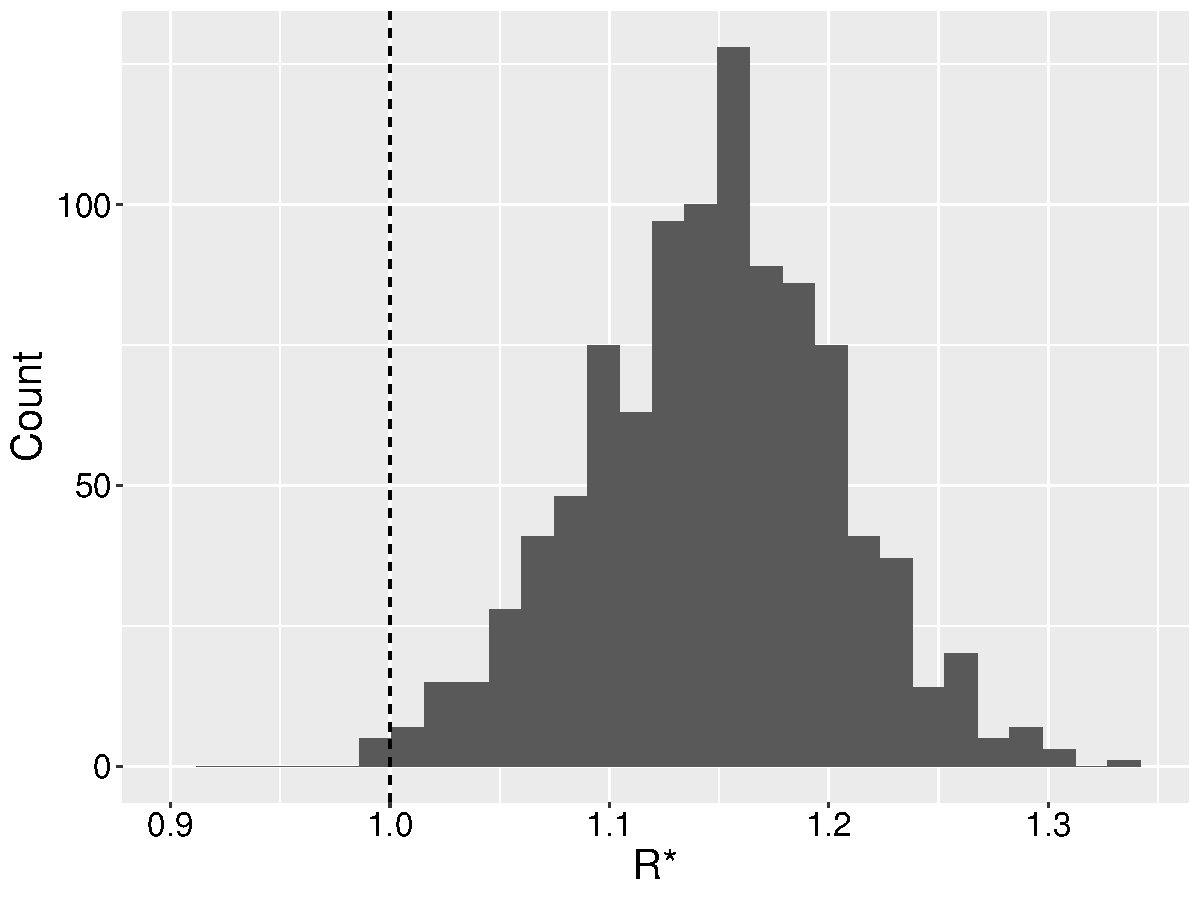
\includegraphics[width=0.6\textwidth]{bivariate.pdf}}
	\caption{\textbf{Bivariate normal example.} The distribution for $R^*$ across 1000 draws.}
	\label{fig:bivariate}
\end{figure}

\subsubsection{250-dimensional model}\label{sec:multivariate_normal_250}
We next consider a more challenging problem -- a 250-dimensional multivariate normal target where its precision matrix, $\boldsymbol{A}\in\mathbb{R}^{250}\times\mathbb{R}^{250}$, is generated from a Wishart distribution \citep{hoffman2014no}. We assume that the Wishart distribution's degrees of freedom is 250, resulting in a distribution with high correlations between dimensions. We use Stan's NUTS algorithm to sample from this target distribution and run the algorithm for two different iteration counts (each time across 4 chains): 400 and 10,000 (the latter thinned by a factor of 5). First, we used Stan to sample from the ``centered'' parameterisation of this model, which is of the form,
%
\begin{equation}\label{eq:mvt_normal_250}
\boldsymbol{x}\sim \mathcal{N}(\boldsymbol{0},\boldsymbol{A}^{-1}),
\end{equation}
%
where $\boldsymbol{x}\in\mathbb{R}^{250}$. For each set of draws, we used Algorithm \ref{alg:R_star_uncertainty} to generate an uncertainty distribution for $R^*$, which is shown in Fig. \ref{fig:mvt}A. From the plot for the 400 iteration case, it is clear that convergence has not yet occurred since $R^*>1$ across the bulk of this distribution. Even in the 10,000 iteration case, the $R^*$ distribution remains stubbornly shifted a little rightwards of $R^*=1$ (its mean is 1.06): in this case, $\widehat{R}<1.01$ for 95\% of parameters (Fig. \ref{fig:mvt}B), although 54\% had bulk-$\text{ESS}<400$ and 13\% of parameters had tail-$\text{ESS}<400$ indicating issues with convergence \citep{vehtari2019rank}.

Rather than run the MCMC sampler for more iterations, we move to a ``non-centered'' parameterisation, which introduces auxillary variables $\boldsymbol{z}\in\mathbb{R}^{250}$ that don't affect $p(\boldsymbol{x})$ but facilitate sampling from it. This model has the form,
%
\begin{align}
\boldsymbol{A}^{-1} = \boldsymbol{L}\boldsymbol{L}^T,\qquad
\boldsymbol{x} = \boldsymbol{L} \boldsymbol{z},\qquad
z_j\sim \mathcal{N}(0, 1), \text{ for } j = 1,2,...,250.
\end{align}
%
where $\boldsymbol{L}$ is the Cholesky decomposition of the covariance matrix, $\boldsymbol{A}^{-1}$. Fig. \ref{fig:mvt}A shows the $R^*$ distribution resultant from 10,000 NUTS iterations in this case: now the distribution has mean $R^*=1.00$. Fig. \ref{fig:mvt}B shows the $\widehat{R}$ values for each $x$ parameter in this model, and, echoing the result for $R^*$, $\widehat{R}<1.01$ in all cases; further, bulk- and tail-$\text{ESS}>400$ for all parameters.

\subsubsection{Variable importance}\label{sec:multivariate_normal_varimportance}
In GBMs, it is possible to calculate variable importance (see, for example, \cite{friedman2001greedy} and \cite{greenwell2019package}), and this allows us to determine which variables were most informative for predictions. We now compare these with the more established metrics $\widehat{R}$ and ESS. For a GBM fitted to the centered model of eq. \eqref{eq:mvt_normal_250} with 10,000 MCMC iterations (thinning by a factor of 5) for each chain, we plot in Fig. \ref{fig:mvt}C variable importance (here high values mean a variable is more important) versus $\widehat{R}$ for all dimensions of the target distribution (including Stan's $lp$ quantity, shown as a triangle). In this plot, there is a positive association between GBM's variable importance and $\widehat{R}$ (Spearman's rank correlation: $\rho=0.33, S=1763958, p<0.01$). In Fig.  \ref{fig:mvt}D, we plot variable importance versus two measures: bulk-ESS and tail-ESS, which both exhibited a strong non-linear negative association (Spearman's rank correlation: bulk-ESS: $\rho=-0.57, S=4142470, p<0.01$; tail-ESS: $\rho=-0.56, S=4113709, p<0.01$). Since none of these plots form perfect ``lines'' along which all the plotted points fall, this illustrates that variable importance provides information complementary to $\widehat{R}$ and ESS.

\begin{figure}[!htb]
	\centerline{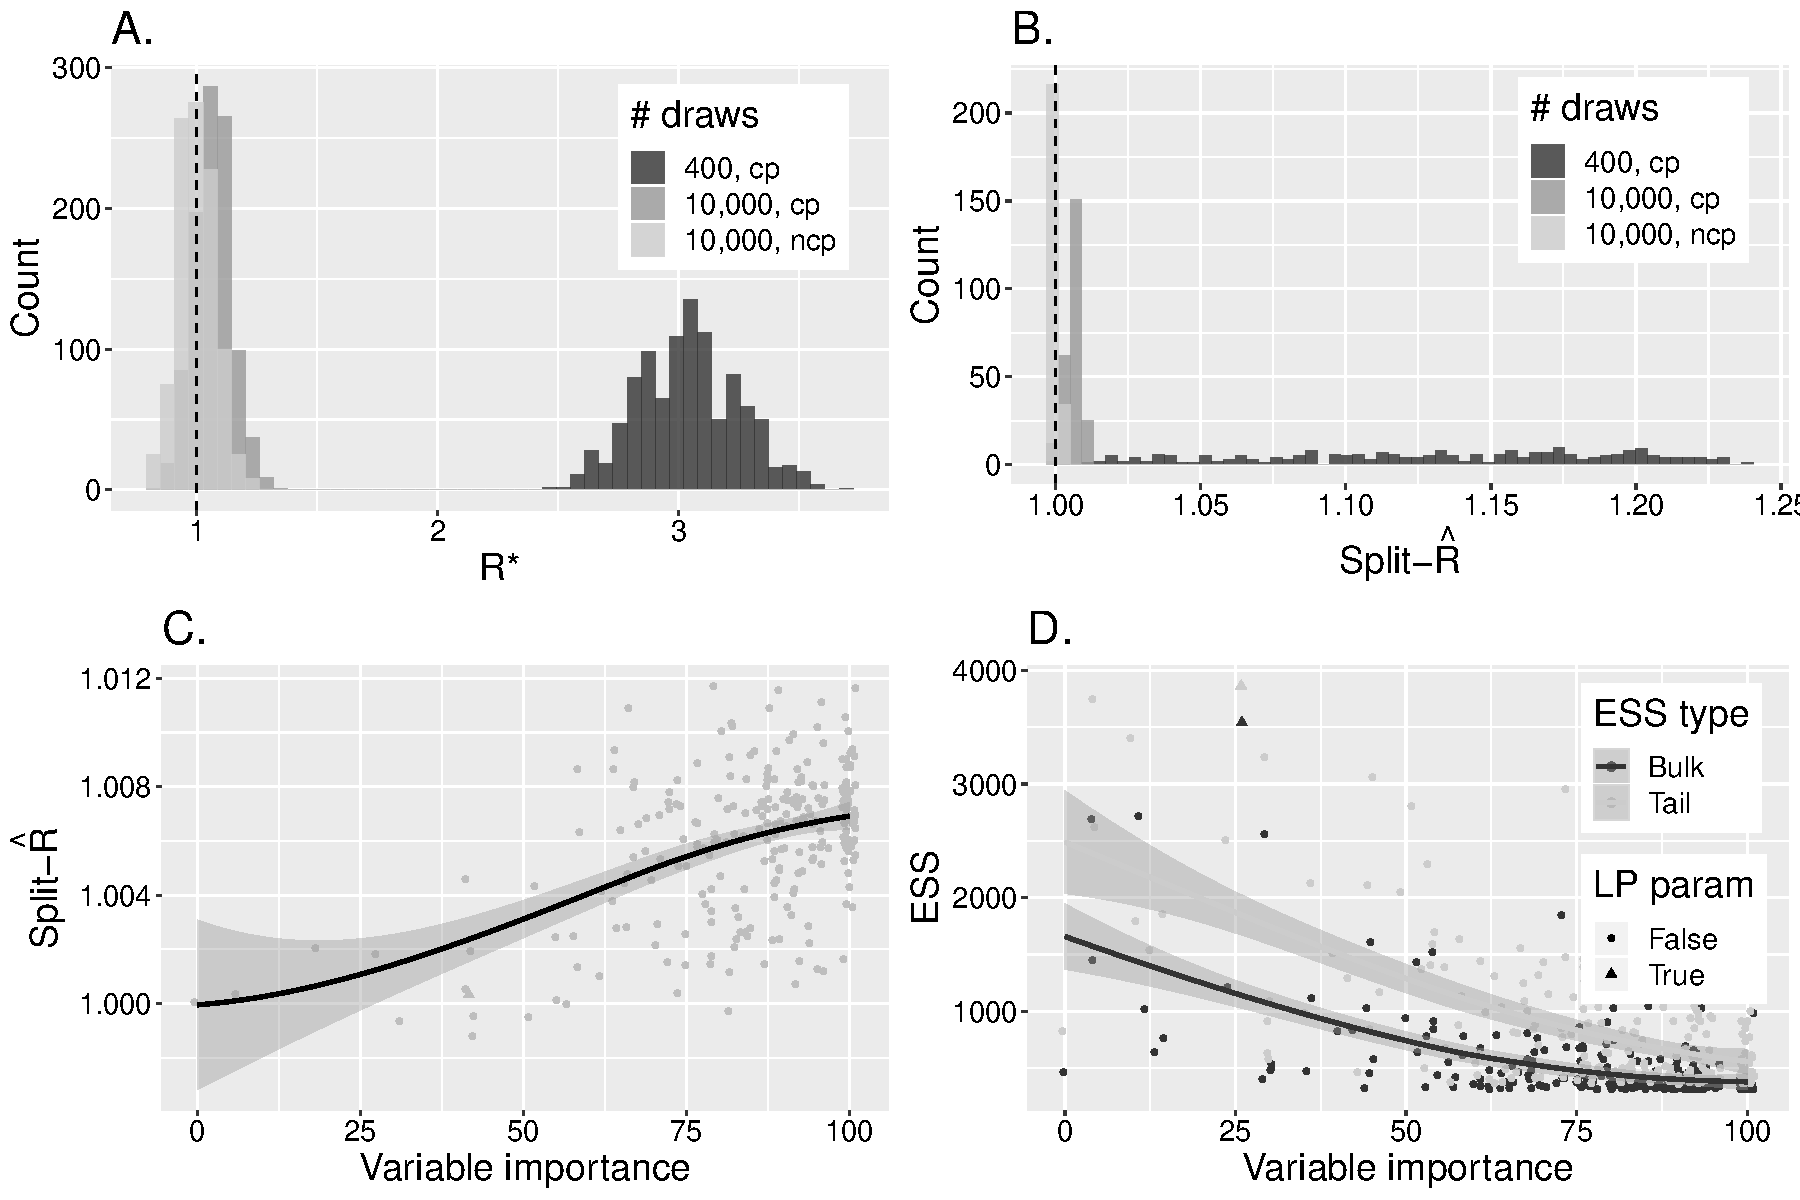
\includegraphics[width=1\textwidth]{mvt_three.pdf}}
	\caption{\textbf{Multivariate normal example with 250 dimensions.} A shows $R^*$ distributions obtained for two MCMC samples (of differing numbers of draws: 400 and 10,000) from the centered parameterisation (``cp'') and one from the non-centered version (``ncp''; with 10,000 draws); B shows the rank-normalised split-$\widehat{R}$ values for all parameters from the same MCMC runs as in A; C shows variable importance versus $\widehat{R}$ for each parameter; and D shows variable importance versus bulk- and tail-ESS as calculated by \cite{vehtari2019rank}. In A, 1000 $R^*$ draws by Algorithm \ref{alg:R_star_uncertainty} are shown for each MCMC run. In plots C and D, horizontal jitter was added to the points and a loess fit line with standard errors overlaid.}
	\label{fig:mvt}
\end{figure}

\subsection{Infinite variance: Cauchy example}\label{sec:cauchy}
We next explore how $R^*$ can be used to determine convergence for distributions with infinite variance. Like \cite{vehtari2019rank}, we first use Stan to sample from independent standard Cauchy distributions for each element of a 50-dimensional vector $x$,
%
\begin{equation}
x_j\sim \text{Cauchy}(0, 1),\; \text{for } j=1,...,50.
\end{equation}
%
We call this parameterisation the ``nominal'' version of this model.

In addition, we also use Stan to sample from an ``alternative'' parameterisation of the Cauchy, based on a scale mixture of Gaussians \citep{vehtari2019rank},
%
\begin{align}
a_j \sim  \N(0,1), \qquad
b_j \sim  \text{Gamma}(0.5, 0.5), \qquad
x_j =  a_j/\sqrt{b_j}.
\end{align}
%
The distribution of the $x$ vector is the same under both parameterisations, although the thin-tailed $(a,b)$ vectors define a higher dimensional posterior that improves sampling efficiency.

In the top-left panel of Fig. \ref{fig:cauchy}, we show the $R^*$ distribution under both parameterisations. As shown in \cite{vehtari2019rank}, the nominal parameterisation results in poor sampling efficiency due to its long tails, meaning that, after 1000 MCMC post-warm-up iterations (with 1000 warm-up iterations discarded) across each of 4 chains, draws still contain information about chain identity, and, accordingly, the $R^*$ distribution is shifted rightwards from $R^*=1$. The alternative parameterisation fares better, and the $R^*$ distribution is nearer $R^*=1$, yet its mean remains above this value. In the top-right panel of Fig. \ref{fig:cauchy}, we show the rank-normalised split-$\widehat{R}$ values across each of the 50 parameters for the same MCMC runs. The nominal parameterisation has some parameters with $\widehat{R}>1.01$, indicative non-convergence, whereas the alternative has $\widehat{R}<1.01$ for all parameters.

Since the $R^*$ distribution indicated non-convergence for both parameterisations, we ran each model for sixty-times as long, although thinned by a factor of 3, resulting in 10,000 post-warm-up iterations across each of 4 chains. In the bottom row of Fig. \ref{fig:cauchy}, we show the results for these longer runs. In these, the alternative parameterisation now has an $R^*$ distribution centered on $R^*=1$ and, hence, we are more confident that convergence has occurred. Despite the added iterations, the $R^*$ distribution from the nominal model remains stubbornly away from 1. The $\widehat{R}$ values are all below 1.01, indicating convergence in both cases.

\begin{figure}[!htb]
	\centerline{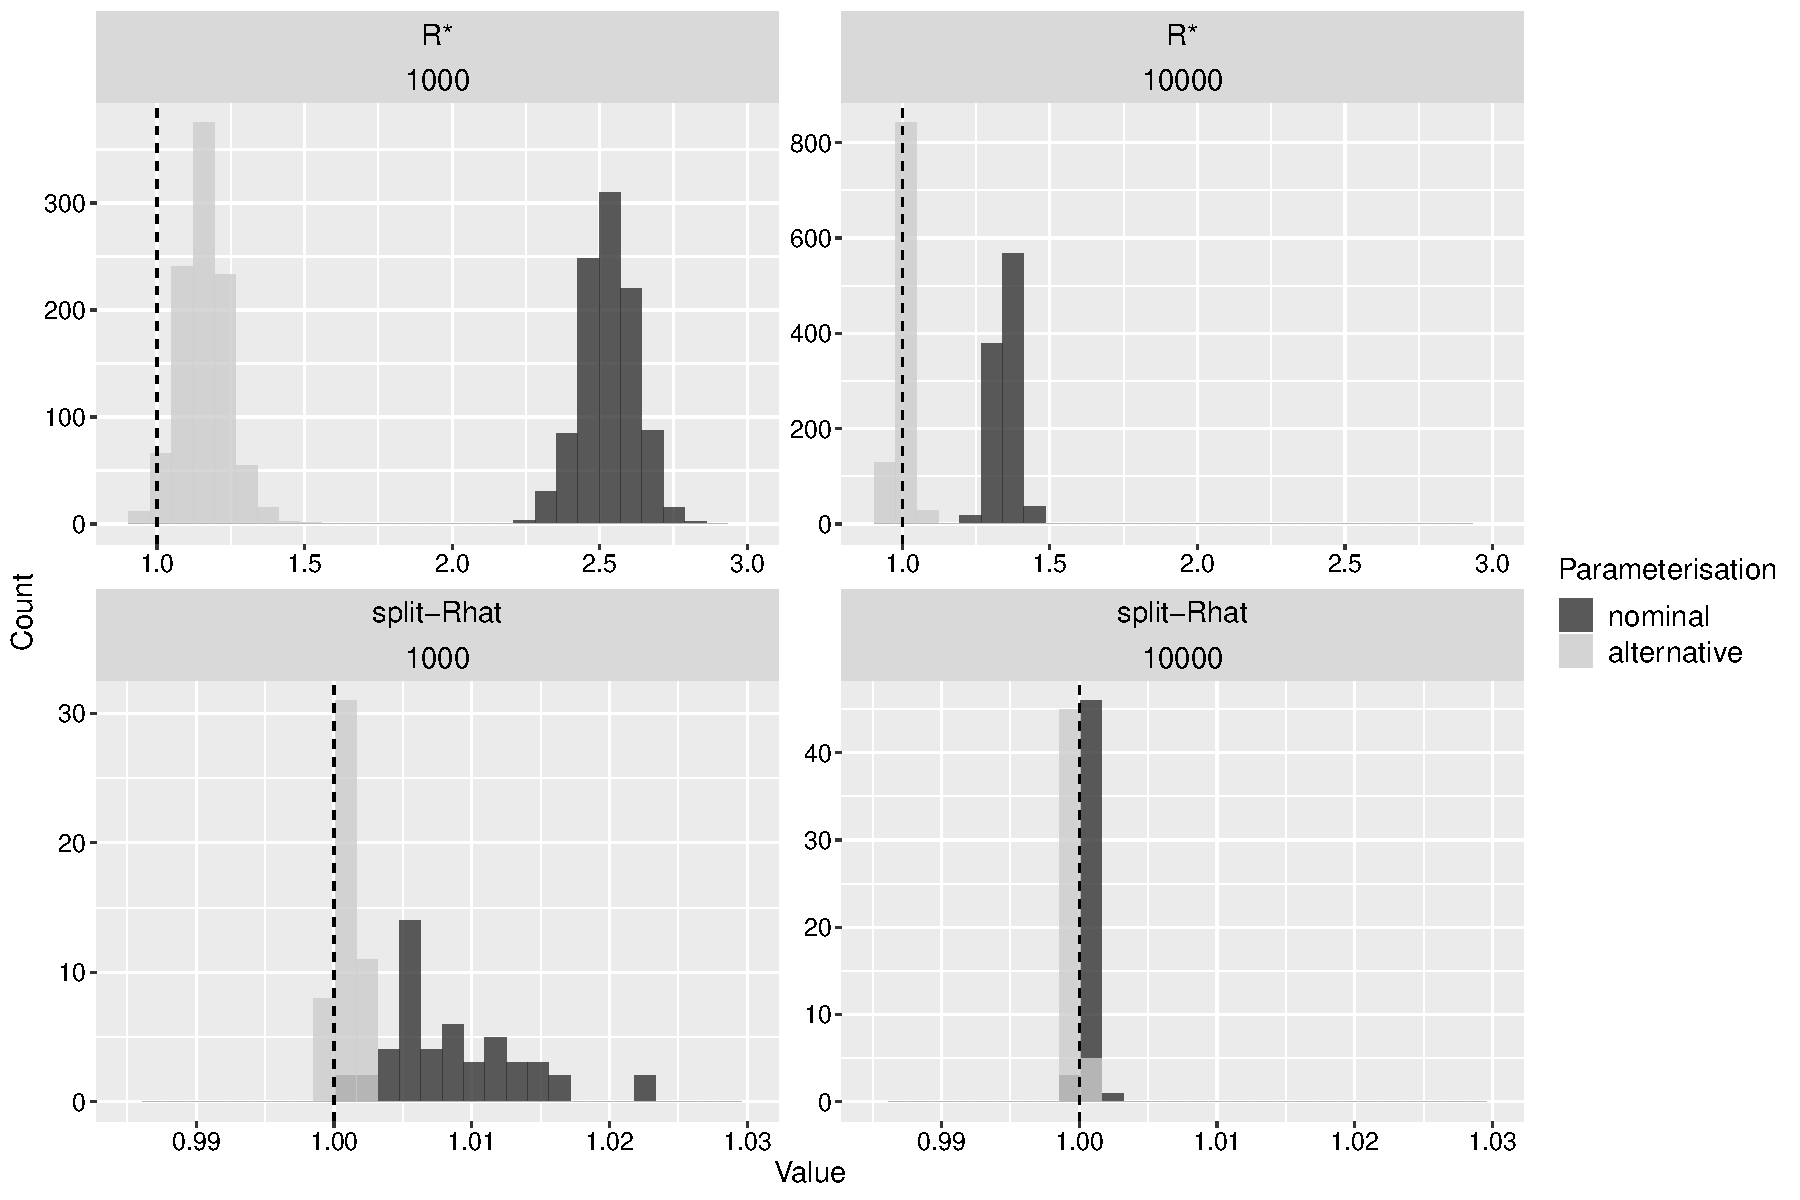
\includegraphics[width=1.0\textwidth]{cauchy.pdf}}
	\caption{\textbf{Cauchy example.} Rows show convergence results for MCMC runs with 1000 (top) and 10,000 (bottom; obtained by thinning iterations by a factor of 3) post-warm-up iterations (each with half iterations discarded as warm-up) for each of 4 chains. Columns show the $R^*$ distributions (left) and rank-normalised split-$\widehat{R}$ values across all parameters (right). Shadings indicate different model paramerisations as indicated in legend.}
	\label{fig:cauchy}
\end{figure}

\subsubsection{Measuring convergence objectively}\label{sec:cauchy_objective}
To illustrate that $R^*$ provides a reliable metric for capturing convergence, we now calculate a quantitative measure that captures how closely a sampling distribution matches the target. One measure of distributional ``closeness'' is the KL-divergence, which, in this case, could be used to measure the divergence from target to sampling distribution: if the target distribution is known, fitting a kernel density estimator (KDE) to samples allows an approximate (typically univariate) measure of KL-divergence to be calculated for each dimension. The trouble is, for distributions like the Cauchy with fat tails, fitting a KDE to the samples provides a noisy measure of the sampling distribution in the tails. This means that approximate KL-divergence is unreliable for these types of model. We decided not to use the Kolmogorov-Smirnov (KS) test, since it is most sensitive to differences between distributions around the median, whereas, here, we are interested in behaviour in the tails. Additionally, we found that the Anderson-Darling and Cram\'er-Von Mises tests \citep{faraway2019goftest}, which do not suffer the same shortcomings as the KS, behaved equally erratically and provided measures that were hard to intuit. The Wasserstein distance was also trialled but had great uncertainty due to the long-tails of the Cauchy. Instead, we chose a measure of distributional discrepancy based around similarity between target quantiles and sample-estimated equivalents. Specifically, we calculate the $R^2$ for the linear regression of actual quantile values on sample-estimated quantiles, where, if $R^2\sim 1$, the sampling distribution recapitulates well the target quantities. In our example, we consider all percentiles: 0.1\%, 0.2\%,...,99.8\%, 99.9\% and calculate the mean $R^2$ across all 50 dimensions.

In Fig. \ref{fig:cauchy_convergence}A, we plot this \textit{quantile-$R^2$} as a function of MCMC sample size for both parameterisations of the Cauchy model. This shows that after c.10,000 iterations, the alternative parameterisation approaches $R^2\approx 1$; at the same number of iterations, the nominal parameterisation still provides a poor measure of tail quantiles. Next, in Figs. \ref{fig:cauchy_convergence}B\&C, we plot two measures of $\widehat{R}$, each calculated from splitting the 4 original chains into two equal halves. The first of these measures is the rank-normalised $\widehat{R}$ \citep{vehtari2019rank}, which provides a separate measurement for each target dimension; in Fig. \ref{fig:cauchy_convergence}B, we show how the maximum of this measurement across all 50 dimensions changes with sample size. After c.550 iterations, the alternative parameterisation achieves $\widehat{R}<1.01$ for all target dimensions, and, after c.10,400 iterations, the nominal model achieves the same maximum $\widehat{R}$ value: in both cases, these suggest convergence. The second measure is multivariate $\widehat{R}$ \citep{brooks1998general}, which, like $R^*$, yields a single measurement across all dimensions; Fig. \ref{fig:cauchy_convergence}C shows how this metric changes with sample size for both Cauchy model parameterisations. After c.1800 iterations, multivariate $\widehat{R}<1.01$ for the alternative parameterisation, whilst after 25,000 iterations multivariate $\widehat{R}>1.07$ indicating more draws are needed. In Fig. \ref{fig:cauchy_convergence}D, we plot $R^*$ against iteration for both models: these indicate that, after 25,000 iterations, $R^*\approx 1.05$ for the alternative model, and $R^*>2$ for the nominal parameterisation: both these $R^*$ values suggest lack of convergence. Finally, in Figs. \ref{fig:cauchy_convergence}E\&F, we plot the minimum across all the dimensions of tail- and bulk-ESS calculated as described in \cite{vehtari2019rank}. After c.180 iterations, the alternative parameterisation surpassed a tail-ESS of 400; after c.18,700, the nominal parameterisation did the same. Both models were quicker to pass 400 bulk-ESSs.

Comparing our ``omniscient'' measure of convergence shown in Fig. \ref{fig:cauchy_convergence}A, with the various derived measures, all show a similar pattern: as sample size increases, the various statistics tend towards convergence. The rate at which these converge differs though, and $R^*$ (Fig. \ref{fig:cauchy_convergence}D) appears at least, qualitatively, most similar to our ``omniscient'' measure.

\begin{figure}[!htb]
	\centerline{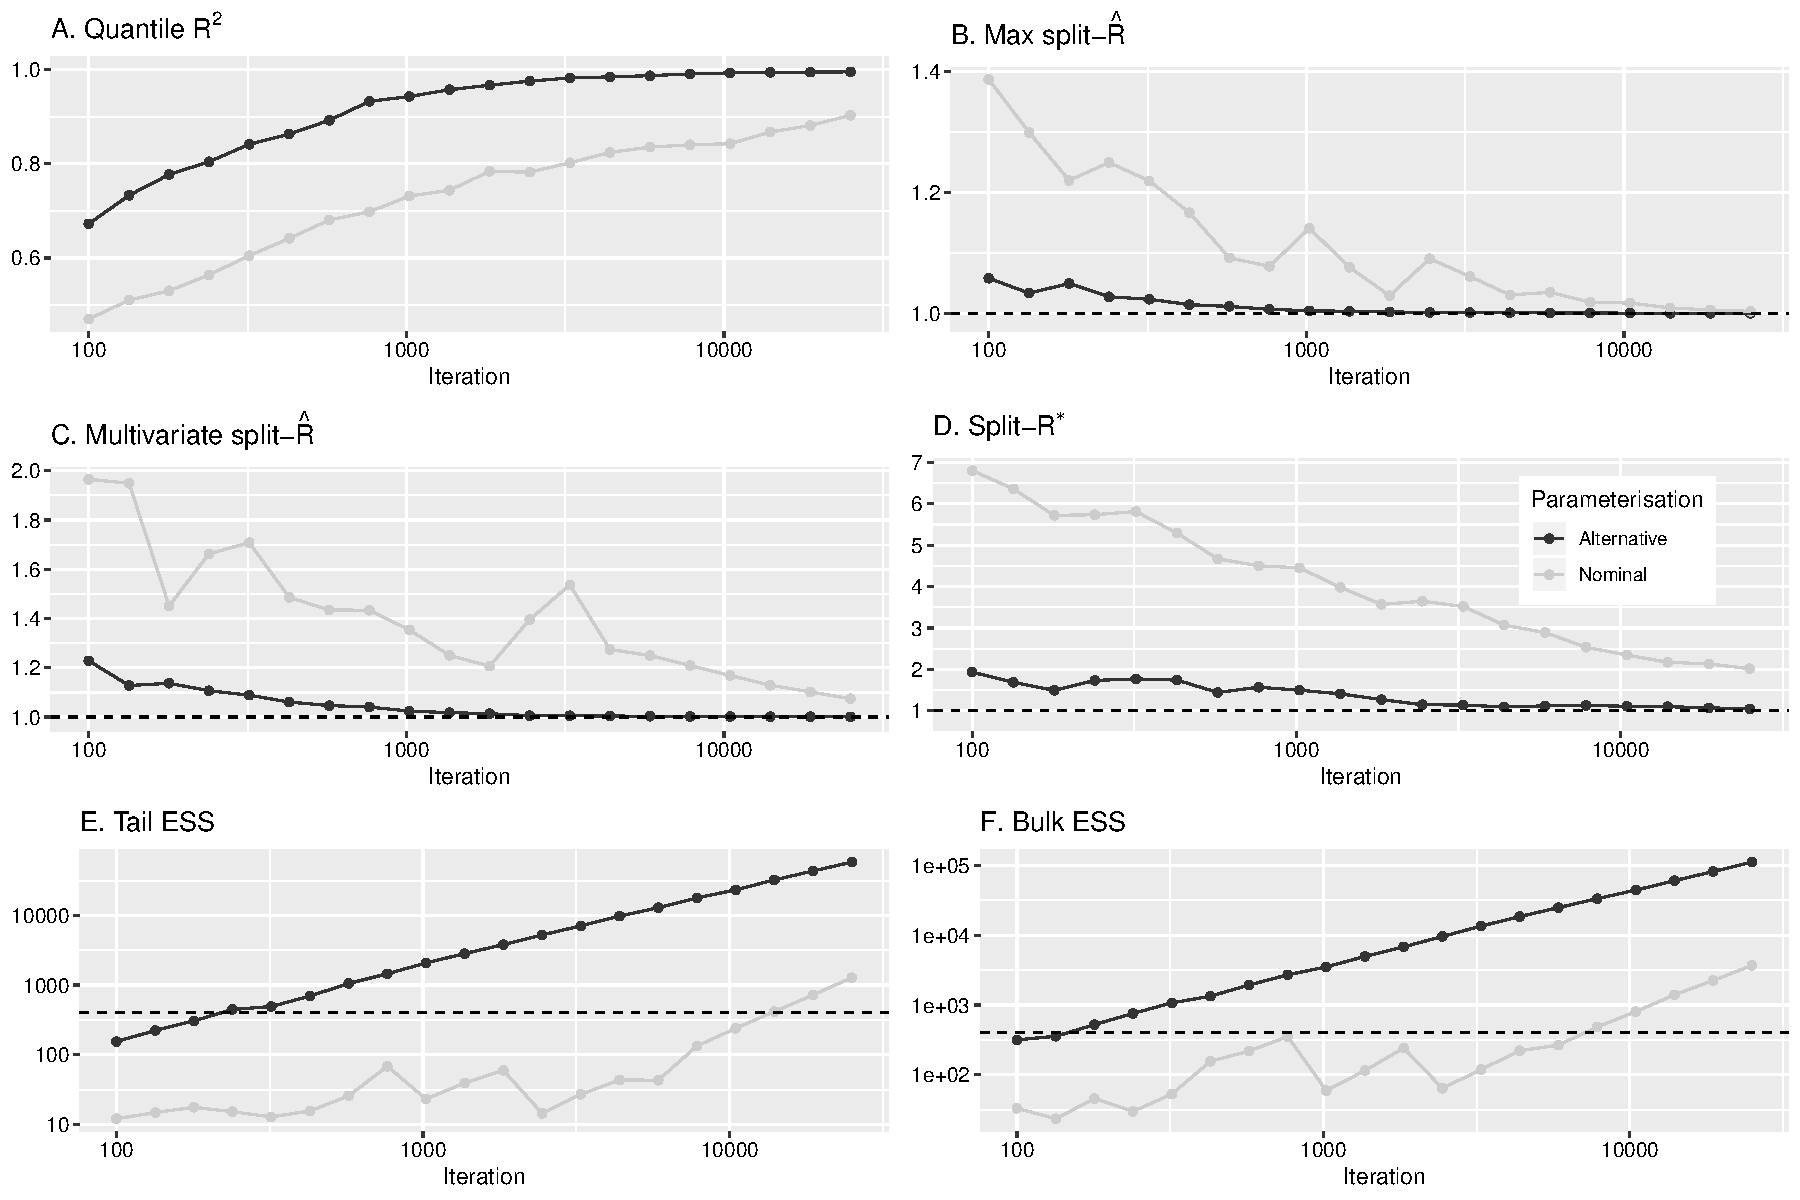
\includegraphics[width=1.0\textwidth]{cauchy_convergence.pdf}}
	\caption{\textbf{Measuring convergence for the Cauchy model.} A shows a measure of convergence, the mean quantile $R^2$, that requires knowing the target distribution; B shows the maximum value of split-$\widehat{R}$ across each of the 50 dimensions of the target; C shows the multivariate split-$\widehat{R}$ value; D shows the value of split-$R^*$ as calculated by Algorithm \ref{alg:R_star}; and E and F show tail- and bulk-ESS. Dashed lines indicate recommended thresholds for each convergence statistic.}
	\label{fig:cauchy_convergence}
\end{figure}

\subsection{Hierarchical model: Eight schools model}\label{sec:eight_shools}
We now examine a classic example used to highlight difficulties in performing inference for hierarchical models: referred to as the ``Eight schools'' model (see Section 5.5 in \cite{gelman2013bayesian}), which aimed to determine the effects of coaching on SAT scores in eight schools. 

The model can be parameterised in two ways, as described in \cite{vehtari2019rank}. The simplest way is referred to as the ``centered'' parameterisation and exactly mirrors the underlying statistical model,
%
\begin{align*}
\theta_j &\sim \N(\mu, \tau), \\
y_j &\sim \N(\theta_j, \sigma_j).
\end{align*}
%
The ``non-centered'' parameterisation recodes this model in a way that does not affect the joint distribution of $(\theta, \mu, \tau, \sigma)$ but makes it easier to sample from it, by introducing auxillary variables, $\tilde \theta_j$. This can be written as,
%
\begin{align*}
\tilde{\theta}_j &\sim \N(0, 1), \\
\theta_j &= \mu + \tau \tilde{\theta}_j,\\
y_j &\sim \N(\theta_j, \sigma_j).
\end{align*}
%
In both cases, $\theta_j$ are the treatment effects in the eight schools, and $(\mu, \tau)$ represent the population mean and standard deviation 
of the distribution of these effects. In the centered parameterization, the $\theta_j$ are parameters, whereas in the non-centered parameterization, the $\tilde{\theta}_j$ are parameters and $\theta_j$ is a derived quantity.

We first used Stan \citep{carpenter2017stan} to sample from the centered model using 4 chains. Like \cite{vehtari2019rank}, we used settings that reduce the chance of divergent iterations for the NUTS algorithm \citep{betancourt2017conceptual}, meaning that the resultant sampling distribution is likely to be biased. We also used the same algorithm settings to sample from the non-centered model.

To see how $R^*$ performed on this example, we first split each of the (post-warm-up) chains in two, as is done by default in Stan \citep{carpenter2017stan} and in \cite{vehtari2019rank}, resulting in 500 iterations across 8 chains. Following the same approach as in Algorithm \ref{alg:R_star_uncertainty}, we generated $R^*$ distributions for both the centered and non-centered models. The resultant distributions for $R^*$ are shown in Fig.\ref{fig:eight_schools}A. In this plot, the centered model is close to convergence, whereas the non-centered is not.

In addition, to illustrate the power of $R^*$, we also repeat the analysis but, this time, do not split the chains in two. The results are shown in Fig.\ref{fig:eight_schools}B. In this case, because the unsplit chains do not mix with themselves, it is harder to accurately predict the chain that generated each draw, meaning that the centered model $R^*$ values are shifted leftwards. Despite this, however, the centered model distribution for $R^*$ still does not strongly overlap with $R^*=1$, indicating that the model has not converged, contrasting with the non-centered model which appears near convergence.

It is recommended that $\widehat{R}$, like $R^*$, be calculated using split chains. In Fig. \ref{fig:eight_schools}C, we plot $\widehat{R}$ values obtained when using the original 4 chains (horizontal axis) versus those when using the split chains (vertical axis) for the ten parameters in this model; we do this for both the centered and non-centered models. These show that the values of $\widehat{R}$ for the centered model for both the split and unsplit cases were, for all but a single parameter, above 1.01, echoing the results for $R^*$; also, like $R^*$, $\widehat{R}$ is higher for the split case. All parameters for the non-centered models were below 1.01, indicating convergence.

\begin{figure}[!htb]
	\centerline{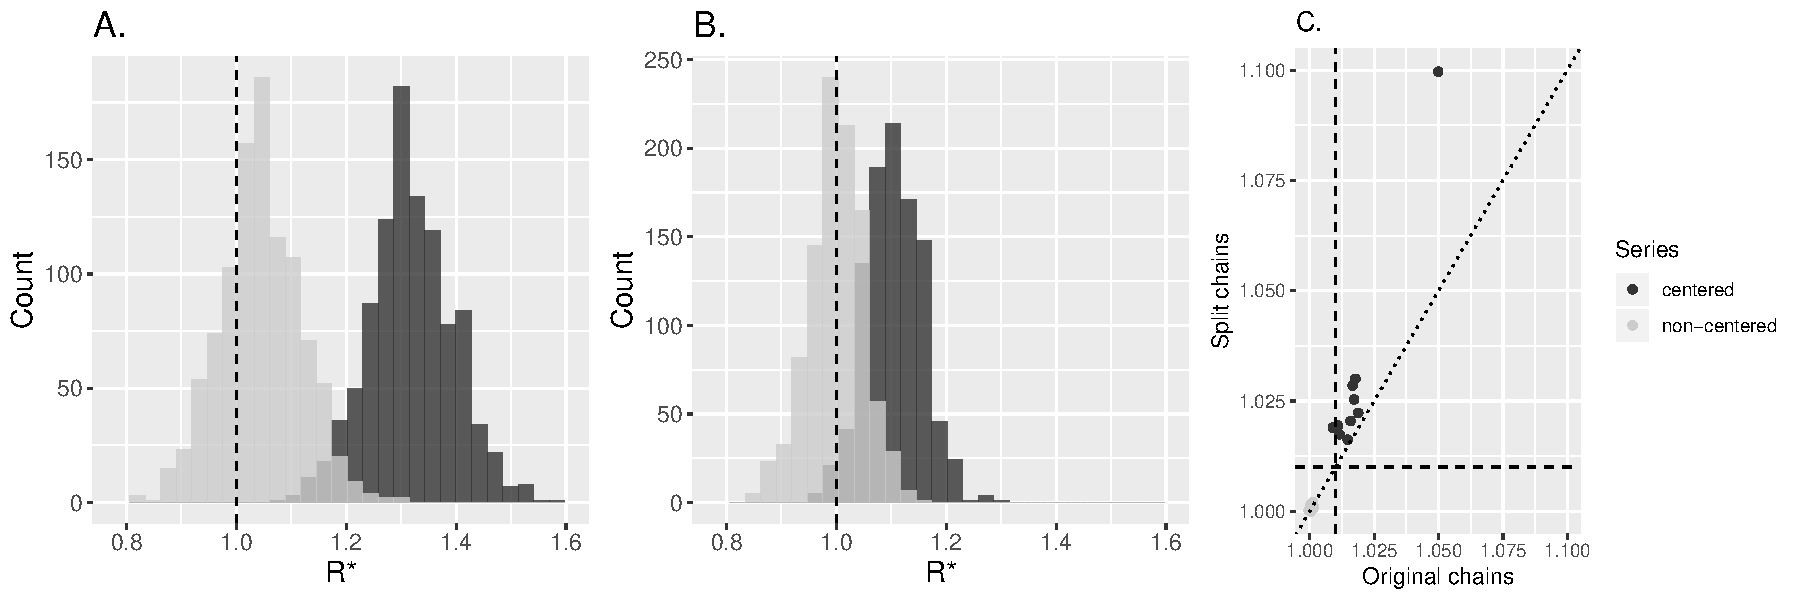
\includegraphics[width=1.0\textwidth]{eight_schools.pdf}}
	\caption{\textbf{Eight schools example: $R^*$ distributions.} A shows draws from the $R^*$ distribution when splitting chains in two (resulting in 8 chains); B shows the same but using the 4 original chains; C shows rank-normalised $\widehat{R}$ for original 4 chains versus those for the 8 chains case for all ten parameters defined by the centered model -- in this case, we plot horizontal and vertical dashed lines to illustrate the $\widehat{R}=1.01$ cutoff and a $y=x$ line. The legend inset in panel C provides a key for all panels. The MCMC samples comprised 2000 draws in all cases, with 1000 used as post-warm-up iterations. In panels A and B, the plots show 1000 $R^*$ draws using Algorithm \ref{alg:R_star_uncertainty} for each parameterisation.}
	\label{fig:eight_schools}
\end{figure}

\subsubsection{Understanding chain classification}
To probe the predictive power of the ML classifier, we investigated how predictive accuracy varies across parameter space. After fitting the GBM model, we group MCMC draws into deciles and draw from the $R^*$ distribution for each decile. In Fig. \ref{fig:eight_schools_r_star_quantiles}, we show the results of this exercise for (A) $\mu$ and (B) $\tau$. In the top row of this figure, we show the path of four MCMC chains (here we did not split chains when calculating $R^*$ to simplify visualisations) across the quantiles of each parameter space. Above the top panel, we show the marginal distributions for each chain. In the bottom row, we show 40 $R^*$ draws for each decile, which were generated according to Algorithm \ref{alg:R_star_uncertainty} using a GBM fit to all draws. In essence, the top rows explain the variation in $R^*$ in the bottom panels: if chains become stuck in regions of parameter space, this causes differences between the marginal distributions of the chains; these differences, in turn, allow a ML model to predict the generative chain in those same sticky regions. For example, for $\mu$, the purple chain became stuck around the middle quantile, forcing a difference in its marginal distribution in that region, which resulted in $R^*>1$ for the corresponding decile. Similarly, for $\tau$, the purple chain became stuck in the lowest quantiles, elevating its marginal distribution there and resulting in improved ML predictive accuracy.

Fig. \ref{fig:eight_schools_r_star_quantiles} also indicates a potential limitation of $R^*$: namely, that as chains are progressively thinned, those regions where chains behave most idiosyncratically can be missed, resulting in a reduction in ML classification accuracy and falsely concluding that convergence has occurred.

\begin{figure}[!htb]
	\centerline{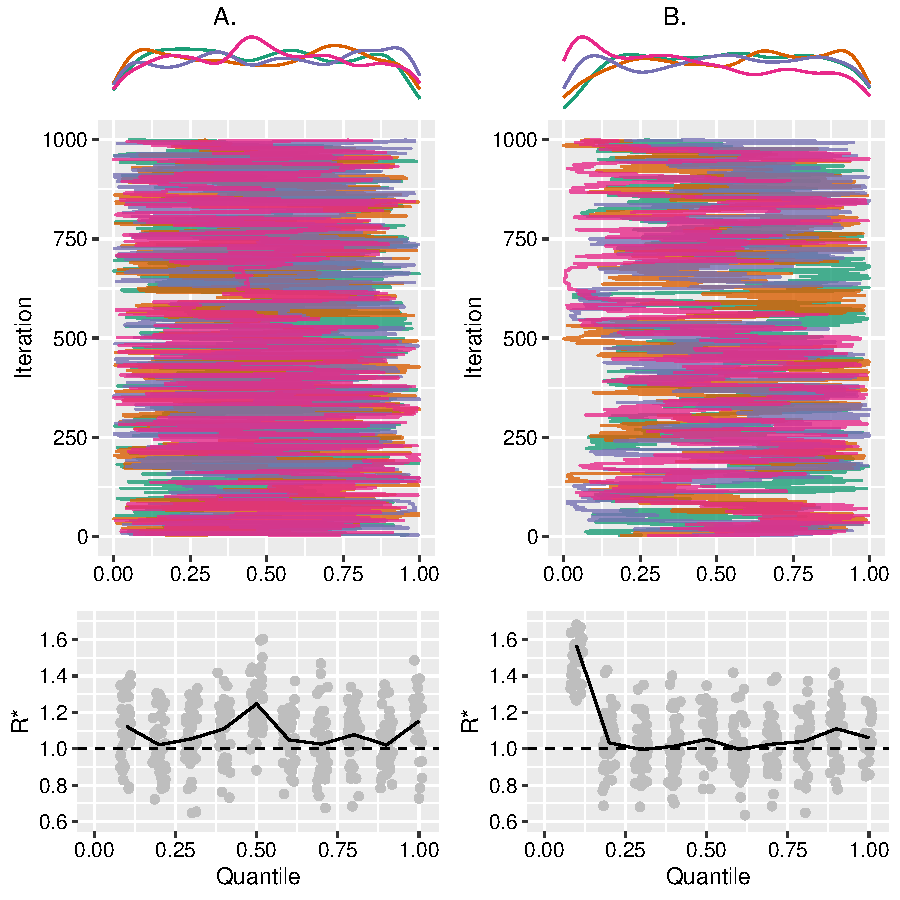
\includegraphics[width=1.0\textwidth]{eight_schools_r_star_quantiles.pdf}}
	\caption{\textbf{Eight schools example: quantile $R^*$ plots.} Column A shows plots for $\mu$; Column B for $\tau$. In each column, we show the path of the four individual chains above and 40 $R^*$ draws obtained using Algorithm \ref{alg:R_star_uncertainty} for each parameter quantile below. Above the top row, we show the marginal distribution of each chain estimated via kernel density estimation using Gaussian kernels. Note that, in the bottom plots, jitter has been added to the data points.}
	\label{fig:eight_schools_r_star_quantiles}
\end{figure}

\subsection{Further experiments}\label{sec:further_experiments}
Alongside the examples included in the main text, there are a number of supplementary text examples, which we briefly outline here.

In \S\ref{sec:wide}, we illustrate how $R^*$ can provide a reasonable measure of convergence when the number of dimensions of a distribution is comparable to the number of draws. Specifically, this was to test that ML classification didn't become prone to overfitting in this limit. To test this hypothesis, we investigated two scenarios using a multivariate normal target: one with a 250-multivariate normal with high correlation between dimensions using 250 post-warm-up iterations; and another normal with 10,000 independent dimensions using up to 500 post-warm-up iterations. In both cases, sampling was done using Stan's NUTS algorithm. In both cases, $R^*$ and rank-normalised split-$\widehat{R}$ reached similar conclusions about convergence: namely, that more iterations were needed in all experiments considered. Overall, these experiments show that $R^*$ is a conservative convergence measure that will tend to diagnose unconvergence when there are insufficient draws.

In \S\ref{sec:non-stationary}, we illustrate the importance of splitting chains before calculating $R^*$ to ensure poor within-chain convergence is diagnosed. We illustrate this via four examples: (a) sampling from a univariate normal and adding a linear trend over sampling time, to ensure that the sampling distributions were non-stationary; (b), similar to (a) but across a range of target distribution dimensions where only a single dimension had a non-stationary mean; (c), a bivariate normal with a non-stationary covariance; and (d), an autocorrelated sampling distribution with a univariate normal target with a range of different autocorrelations. The results of (a) echoed those presented in \cite{vehtari2019rank} for $\widehat{R}$ and showed that $R^*$ is insensitive to sampling non-convergence if it occurs within chains; splitting chains into two halves alleviates this issue. The results of (b) show that $R^*$ calculated on split chains is able to diagnose non-stationarity in mean in a single dimension in a way that did not diminish as the numbers of dimensions considered increased. Example (c) showed that split-$R^*$ opposed to split-$\widehat{R}$ is able to diagnose non-stationary covariance between dimensions of a target distribution. In (d), we show that $R^*$ is able to differentiate between distributions with non-stationary target distributions and stationary ones. It also shows that $R^*$ still functions reasonably at higher levels of chain persistence: yielding a conservative convergence measure when there insufficient draws.

In \S\ref{sec:prostate}, we show that $R^*$ performs well for two Bayesian logistic regression problems with highly multimodal posteriors. Each of these models have 1000s of parameters, and we found that it was slow to compute both $\widehat{R}$ and $R^*$ for them. That said, the computational time for calculating $\widehat{R}$ was considerably less than was needed for $R^*$.


\section{Discussion}
If an MCMC sampler has converged on the target distribution, the chains must be well-``mixed'', that is, given a draw, it should be impossible to discern which chain generated it. Based on this observation, we used supervised machine learning (ML) classifiers to quantify the information about the generative chain identity contained in draws. By taking the ratio of ML model predictive accuracy obtained on an independent test set to the accuracy of a null model (which predicts a chain's identity uniformly at random), this defines our $R^*$ statistic. By extracting ML-predicted chain probabilities from each prediction in the test set, we can additionally generate an uncertainty distribution for $R^*$. Across a range of previously published examples, $R^*$ was shown to be predictive of whether chains had converged.

The predominant methods for diagnosing MCMC convergence rely heavily on looking for between-chain differences in the marginal distributions along each dimension of the target. $R^*$ naturally includes this information in building a model capable of predicting the chain that generated each draw. It also naturally includes information about the joint distribution across all dimensions of the target. Since converged chains should have similar joint distributions (implying similar marginals), any measure of convergence should account for both of these aspects. Indeed, in \S\ref{sec:multivariate_normal}, we show that more established measures may indicate convergence whereas $R^*$ shows otherwise. This is not a sleight on existing measures, more that this illustrates the complementarity of $R^*$ to them.

When first starting to develop $R^*$, it was unclear to us whether \textit{any} metric aligned with a supervised ML method would be overly sensitive to its hyperparameters. With gradient-boosted regression tree models, we found this not to be the case. Indeed, after a little experimenting, we found that a default set of hyperparameters (which we report in \S\ref{sec:method}) sufficed across all our examples: perhaps, because the classification boundaries for this task are unlikely to be very complex compared to (say) machine vision tasks. To ensure maximal predictive capability of any fitted ML model, however, it is prudent to optimise it over choice of hyperparameters, and further work is needed to determine the importance of this step.

In \S\ref{sec:prostate}, we fit Bayesian models with many 1000s of parameters then used $R^*$ to diagnose convergence, finding that $R^*$ was considerably more expensive to calculate than $\widehat{R}$. The computational cost of training GBMs has been suggested to be $\mathcal{O}(N k)$, where $N$ is the number of training data points and $k$ is the number of dimensions of the target \citep{complexity2018}. If so, this suggests that larger models (usually needing more MCMC iterations) may currently be beyond the reach of $R^*$.

Many implementations of $\widehat{R}$ suggest splitting chains in two before calculating it. In a number of examples, we trial this before calculating $R^*$ and find that this approach leads to more accurate chain prediction. We recommend that this practice be adopted whenever $R^*$ is calculated to ensure that this measure is maximised. Additionally, our ML calculation method for $R^*$ makes it possible to include any covariates which may be useful features for prediction, such as an ``iteration block'' indicator variable taking values $1, 2, ..., K$ in each of $K$ blocks of contiguous iterations. If each chain is thoroughly mixed with itself, including this additional information shouldn't change $R^*$; by contrast, if the chains are random walk-like, this information should boost $R^*$.

MCMC enables inference across a wide range of models encountered across the social, biological and physical sciences. Its ease of implementation, however, masks important underlying fragilities in the method. Namely, that unless the chains have converged to a truly stationary distribution, the draws generated are not faithful depictions of the posterior. In this paper, we introduce a new metric, $R^*$, that is especially good at diagnosing poor convergence in the joint sampling distribution -- an area that has received insufficient attention thus far. $R^*$ can straightforwardly be introduced into existing MCMC libraries and could provide a measure of convergence complementary to existing metrics.


\section{Contributions}
BL conceived of the original idea for $R^*$, carried out all analyses and wrote the original draft of the paper. AV reviewed the paper and made a host of recommendations: including suggesting a large range of new case studies on which to trial the method and also suggesting new visualisations for diagnosing how predictive performance depends on parameter quantiles; these collectively widened the scope of the original paper and substantially improved its quality. BL and AV reviewed and edited the draft of the paper.

\bibliographystyle{chicago}
\bibliography{bibliography} 


	
\end{document}
